\chapter{\gkchapter{Constituance et dépendance}{Différentes représentations de la combinaison}}\label{sec:3.4}

\section{De la dépendance à la constituance}\label{sec:3.4.0}

Les arbres de dépendance sont rejetés par certains linguistes sous prétexte qu’ils lient des mots, alors que les relations mettent aussi en jeu des groupes. C’est là une interprétation très réductrice des arbres de dépendances. Nous avons déjà répété à plusieurs reprises que chaque connexion ou dépendance couvre en fait un \hi{ensemble de combinaisons équivalentes} (voir la \sectref{sec:3.2.14} \textit{La connexion et ses instances}). Nous allons montrer dans ce chapitre que les arbres de dépendance induisent naturellement des structures de constituants et qu’inversement, une structure de constituants peut permettre de récupérer une structure de dépendance. Les deux approches sont à notre avis complémentaires et l’analyse d’une phrase complexe nécessite généralement d’\hi{identifier des unités} et de les décomposer (approche de type constituance) autant que de chercher à \hi{lier entre elles des unités} déjà identifiées (approche de type dépendance).

Notons encore que nous introduisons, dans ce chapitre, \hi{deux types d’arbres} \hi{de constituants}, qu’il est parfois difficile de distinguer, car ils utilisent exactement le même formalisme de représentation. Ces deux arbres, l’\textstyleTermes{arbre de constituants plat} (\sectref{sec:3.4.4})\textstyleTermes{ }et l’\textstyleTermes{arbre de constituants binaire} (\sectref{sec:3.4.14}), sont définis selon des principes différents et la correspondance avec les structures de dépendance permet de mieux comprendre ce qui les distingue. D’autres structures, équivalentes à l’un ou l’autre de ces arbres de constituants, sont également introduites.

\section{ Arbre à la Beauzée-Gladkij}\label{sec:3.4.1}

Reprenons l’exemple introduit à la \sectref{sec:3.3.30} \textit{Dominance et projections maximales} :

\ea\label{ex:laponie2} \textit{Beaucoup de gens aimeraient passer Noël en Laponie.} \z

Nous donnons à nouveau son arbre de dépendance dans la figure \ref{fig:laponie-dep2}.

\begin{figure}
\begin{forest}for tree={font=\itshape,edge=-{Triangle[]}}
[aimeraient
  [beaucoup [de [gens]]]
  [passer 
    [Noël]
    [en [Laponie]]
  ]
]
\end{forest}

\caption{\label{fig:laponie-dep2}Arbre de dépendance}

\end{figure}

Dans un arbre de dépendance, les dépendances sont représentées par des \hi{liens entre des mots}. Ces liens, qui suggèrent la combinaison entre  le mot gouverneur et le mot dépendant, \hi{ne sont qu'une des instances de la dépendance}, qui en tant que connexion hiérarchisée représente un ensemble de combinaisons (voir la \sectref{sec:3.2.14} sur \textit{La connexion et ses instances}). Parmi les instances de la dépendance, il y en a une autre qui est importante, la \hi{combinaison entre le mot gouverneur et la projection maximale du mot dépendant} (voir la \sectref{sec:3.3.30} sur \textit{Dominance et projections maximales} pour la définition de la projection, ainsi que l’\encadref{sec:3.3.31}).

Dans notre exemple, \textit{aimeraient} a pour dépendant \textit{beaucoup} et \textit{passer}. Mais qui \textit{aimeraient passer Noël en Laponie} ? \textit{Beaucoup de gens.} Et ce que \textit{beaucoup de gens aimeraient}, ce n’est pas juste \textit{passer}, mais bien \textit{passer Noël en Laponie}. Ainsi les deux dépendances qui partent de \textit{aimeraient} doivent-elles être vues avant tout comme des dépendances vers les groupes \textit{beaucoup de gens} et \textit{passer Noël en Laponie~}, comme le montre la figure \ref{fig:laponie-groupe}.

\begin{figure}
\begin{tikzpicture}[>={Triangle[]}]
\node at (0,0) [ConcSet,font=\small] (A) {\textit{beaucoup de gens}};
\node [ConcSet,right=.5cm of A,font=\small] (B) {\textit{aimeraient}};
\node [ConcSet,right=.5cm of B,font=\small] (C) {\textit{passer Noël en Laponie}};          

\path[->] (B) edge [bend right] (A)
              edge [bend left] (C);
\end{tikzpicture}
\caption{\label{fig:laponie-groupe}Lien entre le mot \textit{aimeraient} et les projections de ses dépendants}
\end{figure}

Cette \hi{double interprétation du dépendant}, \hi{comme mot et comme groupe}, est déjà bien dégagée par Nicolas Beauzée dans l’article \textit{Régime} de l’Encyclopédie de \citeyear{Beauzée1765} (voir l’\encadref{sec:3.3.2} sur l’\textit{Historique des notions de dépendance et de tête}). Elle est aussi sous-jacente chez Lucien Tesnière, qui considère la dépendance comme une relation entre mots («~dans la phrase \textit{mon ami parle}, \textit{mon} dépend de \textit{ami}, qui dépend à son tour de \textit{parle}~» ; 1959 : chapitre 2), instancie les nœuds par des mots dans ses stemmas, mais définit pourtant le nœud «~comme l’ensemble constitué par le régissant et par tous les subordonnés qui, à un degré quelconque directement ou indirectement, dépendent de lui et qu’il noue ainsi en quelque sorte en un seul faisceau~» \citep[chapitre 3]{tesniere1959elements}.
 
Cette ambivalence du dépendant trouve sa première interprétation graphique avec la représentation proposée par Aleksej Gladkij en \citeyear{gladkij1968describing}, où les projections sont explicites (voir figure \ref{fig:laponie-gladkij}).

\begin{figure}
\begin{tikzpicture}[
                     every node/.style={font=\itshape\strut, inner sep=5pt}, 
                     edge from parent/.style={draw,-{Triangle[sep=1.5pt]}},
                     level 1/.style={sibling distance=30mm},
                     level 2/.style={sibling distance=15mm},
                     level 3/.style={sibling distance=7mm}
                   ]
  \node (root) {aimeraient}
    child { node {beaucoup}
            child { node {de} 
                child { node [draw,rounded corners=2pt] {gens} } 
                  }
          }
    child { node { passer }
             child { node [draw,rounded corners=2pt] { Noël } }
             child { node { en }
                     child { node [draw,rounded corners=2pt] { Laponie } } }
           };
\begin{scope}[every node/.style={draw, inner sep=1pt, rounded corners=2pt}]
\node [fit = (root-2-2) (root-2-2-1)] (enLaponie) {};
\node [fit = (root-1-1) (root-1-1-1)] (degens) {};
\node [fit = (root-1) (degens)] (beaucoupdegens) {};
\node [fit = (root-2) (root-2-1) (enLaponie)] (passerNoelenLaponie) {};
\end{scope}
\end{tikzpicture}
\caption{\label{fig:laponie-gladkij}Arbre de Beauzée-Gladkij}
\end{figure}
\todo[inline]{In this figure, boxes are really part of the structure, they are nodes in the "tree". In other words, the space below the edges must be widened. }
\todo[inline]{A box around the whole structure is missing.}
\todo[inline]{The space between the boxes could be widened, as in the next figure, which is nice. In some sense, the next figure is the same figure without the edges.}

Cette représentation, que nous appellerons désormais un \textstyleTermes{arbre de Beauzée-Gladkij}, n’est pas un arbre au sens mathématique du terme, mais un arbre à bulles (voir l’\encadref{sec:3.2.23} \textit{Graphe à bulles et polygraphe}) : les dépendants ne sont plus des nœuds élémentaires, mais des ensembles de nœuds, représentés par des bulles. Si l’on compare l’arbre de Beauzée-Gladkij avec l’arbre de dépendance, on voit que chaque nœud a été remplacé par sa \hi{projection maximale}. Laquelle projection est elle-même analysée, avec un nœud tête dont dépendent des projections, et ainsi de suite.

On aura noté que \hi{l’arbre} \hi{de Beauzée-Gladkij} \hi{est absolument équivalent à l’arbre} \hi{de dépendance}. Il ne contient aucune information supplémentaire, il ne fait qu’expliciter les projections maximales, qui étaient déjà implicitement présentes dans l’arbre de dépendance.

\section{Arbre de constituants plat}\label{sec:3.4.2}

L’arbre de Gladkij induit lui-même une nouvelle structure. Oublions les dépendances et gardons uniquement les projections maximales : on obtient alors uniquement un \hi{emboîtement} d’unités. 

\begin{figure}
\begin{tikzpicture}[every node/.style={font=\strut,inner sep=1pt}]
 \matrix (matrix) [matrix of nodes,column sep=1em]
    {beaucoup & de & gens & [7pt] aimeraient & passer & Noël & en & Laponie\\};
\begin{scope}[every node/.style={draw,rounded corners=2pt}]
 \node [fit = (matrix-1-3), inner sep=2pt] (gens) {};
 \node [fit = (matrix-1-6), inner sep=2pt] (Noel) {};
 \node [fit = (matrix-1-8), inner sep=2pt] (Laponie) {};
 
 \node [fit = (matrix-1-7) (Laponie), inner sep=3pt] (enLaponie) {};
 \node [fit = (matrix-1-2) (gens), inner sep=3pt] (degens) {};
 
 \node [fit = (matrix-1-1) (degens), inner sep=4pt] (beaucoupdegens) {};
 \node [fit = (matrix-1-5) (enLaponie), inner sep=4pt] (passerenLaponie) {};
 
 \node [fit = (beaucoupdegens) (passerenLaponie), inner sep=5pt] {};
\end{scope}
\end{tikzpicture}
\caption{\label{fig:laponie-box}Emboîtement (de constituants majeurs)}
\end{figure}

Il est d’usage d’appeler les unités dans une telle structure les constituants (voir l’\encadref{sec:3.4.3} sur \textit{Le terme} constituant).

\Definition{\textstyleTermes{structure de constituants}, \textstyleTermes{constituant}, \textstyleTermes{constituant majeur}}
{Une structure représentant un emboîtement d'unités syntaxiques est appelée une \textstyleTermes{structure de constituants}. Les unités considérées dans une telle structure sont appelées les \textstyleTermes{constituants}. Les constituants qui correspondent aux \hi{projections maximales} sont appelés les \textstyleTermes{constituants majeurs}.}

L'emboîtement de la figure \ref{fig:laponie-box} peut être représenté sous la forme d’un \hi{parenthésage}.

\begin{figure}
     ( [ \textit{beaucoup} ( \textit{de} [ \textit{gens} ] ) ] \textit{aimeraient} [ \textit{passer} ( \textit{Noël} ) ( \textit{en} [ \textit{Laponie} ] ) ] )
\caption{\label{fig:laponie-parenthese}Parenthésage (de constituants majeurs)}

\end{figure}

Notons néanmoins que le parenthésage ne peut être défini que sur une suite ordonnée d’éléments. Bien que nous ayons représenté l’emboîtement ci-dessus en remettant les mots dans l’ordre de la phrase, nous ne nous intéressons pas à l’ordre linéaire pour l’instant et un emboîtement de constituants peut être considéré indépendamment de l’ordre des mots.

Notre structure de constituants peut encore être représentée d’une autre façon : sous la forme d’un \hi{arbre} (voir l'\encadref{sec:1.2.3} \textit{Graphe et arbre}), que nous appellerons l’\textstyleTermes{arbre de constituants plat}, car il ne contient que les constituants majeurs et il est donc \hi{le plus plat des arbres de constituants que l’on peut considérer}. Nous les représentons selon l’usage avec les mots dans l’ordre linéaire, mais \hi{nous ne nous intéressons} pour l’instant \hi{qu’à} \hi{la structure d’arbre}, c’est-à-dire la structure hiérarchique définie par l’arbre (l’ordre sera considéré au chapitre suivant, voir notamment l’\encadref{sec:3.5.28} sur l'\textit{Arbre de constituants ordonné}).

\begin{figure}
\begin{forest} for tree={font=\itshape,fit=band}
 [\Boite, calign=child, calign primary child=2
    [\Boite
        [beaucoup] [\Boite
            [de] [\Boite
                [gens]
            ]
        ]
    ]
    [ aimeraient ]
    [ \Boite, calign=child, calign primary child=2 
        [passer] [\Boite [Noël]] [\Boite
            [en] [\Boite [Laponie]]
        ]
    ]
 ]
\end{forest}
\caption{\label{fig:}Arbre de constituants plat}
\end{figure}

C’est le mathématicien Yves Lecerf, qui a le premier construit un tel arbre, en \citeyear{lecerf1960programme}, immédiatement après la publication de l’ouvrage de Tesnière en \citeyear{tesniere1959elements}, et qui a établi l’équivalence entre les arbres de dépendance et cette sous-famille d’arbres de constituants. Il est facile de voir que l’arbre de constituants plat est équivalent à l’arbre de Beauzée-Gladkij : chaque nœud étiqueté d’un {\Boite} représente une boîte, dont les constituants sont les fils dans l’arbre. Les branches de cet arbre sont donc à lire comme des \textstyleTermes{relations partie-tout} et non plus comme des relations de dépendance.

\chevalier[sec:3.4.3]{Le terme 	extit{constituant}}{%
    Le terme \textit{constituant} a été introduit par Leonard Bloomfield en 1933 dans son ouvrage \textit{Language}. Bloomfield s’intéresse à la décomposition des unités et il utilise le terme pour désigner les \textstyleTermes{constituants immédiats}  d’une unité (voir la \sectref{sec:3.2.25} \textit{Analyse en constituants immédiats}). Au départ, le terme est donc prédicatif : un constituant est toujours \hi{le constituant immédiat d’une} \hi{autre unité} (il \hi{constitue} une partie de cette unité). Ensuite, le terme a été utilisé pour désigner l’ensemble des unités obtenues par l’analyse en constituants immédiats. Le terme n’est plus prédicatif : \hi{un constituant est devenu un type d’unité}. C’est dans ce dernier emploi que nous utilisons le terme constituant. Nous considérons plusieurs types de constituants : les constituants majeurs, qui sont les projections maximales (voir \sectref{sec:3.4.2}), auxquels s’ajoutent des constituants intermédiaires obtenus par l’analyse en constituants immédiats (voir \sectref{sec:3.4.14} \textit{Arbre de constituants binaire}).

    La conséquence de ce choix terminologique est que, pour désigner les unités qui résultent de la décomposition d’un constituant C, on parle aujourd'hui de \textstyleTermes{sous-constituants} de C (et non plus de constituants immédiats de C).
}
\section{Arbre de constituants avec têtes}\label{sec:3.4.4}

Un arbre de constituants plat possède une propriété particulière : chaque nœud intérieur (correspondant donc à une boîte) possède parmi ses fils un \hi{unique nœud} \hi{terminal} — une feuille de l’arbre. (Dans notre exemple, les nœuds terminaux sont occupés par des mots, car nous avons décidé de ne pas poursuivre la décomposition au-delà. Ce choix est indépendant de la discussion présente qui reste valable quelle que soit la granularité de notre analyse.) Cette propriété d’unicité permet d’interpréter ce \hi{nœud} \hi{terminal} comme la \hi{tête du constituant}. L’arbre de constituants plat est donc implicitement un \textstyleTermes{arbre de constituants avec têtes}.

Il est d’usage dans les arbres de constituants avec têtes (plats ou pas) d’expliciter laquelle des relations partie-tout entre ce constituant et ses sous-constituants est la relation avec la tête. Cela est indiqué par un T dans l'arbre de la figure \ref{fig:laponie-Tplat}. Un arbre de constituant avec têtes est dit \textstyleTermes{plat} lorsque la tête de chaque constituant est un nœud terminal. Nous contrasterons ce type d’arbre avec les arbres X-barre et les arbres de l’analyse en constituants immédiats, qui peuvent être enrichis de têtes, mais sont binaires et non pas plats (voir la \sectref{sec:3.4.14} sur l’\textit{Arbre de constituants binaire}). Nous présentons à cette occasion une autre convention pour l’encodage de la tête dans l’\encadref{sec:3.4.19} sur la \textit{Syntaxe X-barre}.

\begin{figure} \label{fig:laponie-Tplat}
\begin{tikzpicture}[every node/.style={font=\strut}]
\begin{scope}[
    every node/.style={CircleFillNode},
    level 1/.style={sibling distance=30mm},
    level 2/.style={sibling distance=20mm},
    level 3/.style={sibling distance=15mm}
    ]
\node (root) {}
    child { node { } 
        child { node { } edge from parent node [reset shape, midway,anchor=base east] {T} }
        child { node { } 
            child { node { } edge from parent node [reset shape, midway,anchor=base east] {T} }
            child { node { } }
        }
    }
    child { node { } edge from parent node [reset shape, midway,anchor=east] {T}  }
    child { node { }
        child { node { } edge from parent node [reset shape, midway,anchor=base east] {T} }
        child { node { } }
        child { node { } 
            child { node { } edge from parent node [reset shape, midway,anchor=base east] {T} }
            child { node { } }
        }
    };
\end{scope}
\begin{scope}[every node/.style={font=\itshape}]
\node[below=1pt of root-1-1] {beaucoup};
\node[below=1pt of root-1-2-1] {de};
\node[below=1pt of root-1-2-2] {gens};
\node[below=1pt of root-2] {aimeraient};
\node[below=1pt of root-3-1] {passer};
\node[below=1pt of root-3-2] {Noël};
\node[below=1pt of root-3-3-1] {en};
\node[below=1pt of root-3-3-2] {Laponie};
\end{scope}
\end{tikzpicture}

\caption{\label{fig:}Arbre de constituants plat avec explicitation des têtes}
\end{figure}

\section{Equivalence par la méthode de Lecerf}\label{sec:3.4.5}

L’arbre de constituants plat est équivalent à l’arbre de Beauzée-Gladkij et donc à l’arbre de dépendance dont nous sommes partis. Pour reconstruire l’arbre de dépendance, rien n’est plus simple : il suffit d’identifier chaque nœud intérieur avec son nœud tête, comme le montre le diagramme de la figure \ref{fig:laponie-lecerf}. Les nœuds qui vont fusionner sont dans un même cadre gris dans la partie haute et remplacer par un unique nœud dans la partie basse.

\begin{figure}
\fbox{\begin{tikzpicture}[every node/.style={font=\small\strut}]
\begin{scope}[
    every node/.style={CircleFillNode},
    level 1/.style={sibling distance=30mm},
    level 2/.style={sibling distance=15mm},
    level 3/.style={sibling distance=15mm}
    ]
\node (root) {}
    child { node { }
        child [missing]
        child { node { } edge from parent node [reset shape, midway,anchor=east] {T} }
        child { node { }
            child [missing]
            child { node { } edge from parent node [reset shape, midway,anchor=east] {T} }
            child { node { } }
        }
    }
    child { node { } edge from parent node [reset shape, midway,anchor=east] {T}  }
    child { node { }
        child [missing]
        child [missing]
        child { node { } edge from parent node [reset shape, midway,anchor=east] {T} }
        child { node { } }
        child { node { } 
            child [missing]
            child { node { } edge from parent node [reset shape, midway,anchor=east] {T} }
            child { node { } }
        }
    };
\end{scope}
\begin{scope}[every node/.style={font=\itshape}]
\node[below=1pt of root-1-2] (beaucoup) {beaucoup};
\node[below=1pt of root-1-3-2] (de) {de};
\node[below=1pt of root-1-3-3] (gens) {gens};

\node[below=1pt of root-2] (aimeraient) {aimeraient};

\node[below=1pt of root-3-3]   (passer) {passer};
\node[below=1pt of root-3-4]   (Noel) {Noël};
\node[below=1pt of root-3-5-2] (en) {en};
\node[below=1pt of root-3-5-3] (Laponie) {Laponie};
\end{scope}
\begin{scope}[
        on background layer,
        every node/.style={fill=black!20,inner sep=1pt,rounded corners=2pt}, 
        ]
\node [fit = (root) (aimeraient)] {};
\node [fit = (root-3-5-3) (Laponie)] {};
\node [fit = (root-1-3-3) (gens)] {};
\node [fit = (root-3-4) (Noel)] {};
\node [fit = (root-1) (beaucoup)] {};
\node [fit = (root-1-3) (de)] {};
\node [fit = (root-3) (passer)] {};
\node [fit = (root-3-5) (en)] {};
\end{scope}
\end{tikzpicture}}%
\smallskip\\
{\huge$\Downarrow$}
\medskip\\
\fbox{\begin{forest} for tree = {fill=black!20,rounded corners=2pt,font=\itshape}
[aimeraient
  [beaucoup [de [gens]]]
  [passer
    [Noël]
    [en [Laponie]]
  ]
]
\end{forest}}
\caption{\label{fig:laponie-lecerf}Retour à l’arbre de dépendance}
\end{figure}


Au final, nous avons montré la parfaite \hi{équivalence entre} un \hi{arbre de dépendance} et un \hi{arbre de constituants plat}. La méthode que nous avons utilisée pour passer de l’un à l’autre, dans un sens comme dans l’autre est due initialement à Lecerf. Nous appellerons cette méthode la \textstyleTermes{méthode de Lecerf} ou \textstyleTermes{méthode par agrégation des projections}.

\section{ Construire un arbre de dépendance par décomposition}\label{sec:3.4.6}

Dans les chapitres \ref{sec:3.2} et \ref{sec:3.3}, nous avons montré comment construire l’arbre de dépendance d’un énoncé en construisant d’abord une structure de connexion, puis en raffinant et hiérarchisant cette structure grâce à différents critères permettant d’identifier les têtes des unités.

Une autre méthode consiste à construire d’abord un arbre de constituants. Cette méthode suppose qu’on ait repéré l’unité maximale que l’on veut analyser (ce qui n'est pas sans difficulté comme nous le verrons dans la partie 6). Appelons cette unité une phrase selon l’usage. Voici la méthode.

A chaque étape, on a une unité U à décomposer. À la première étape, il s’agit de la phrase que l’on veut analyser. Pour décomposer U, on doit d’abord \hi{repérer la tête} de U (les critères restent les mêmes que ceux que nous avons présentés dans le \chapref{sec:3.3}). On enlève alors cette tête et on regarde ce que sont les morceaux qui restent. Autrement dit, on repère les \hi{sous-unités} \hi{maximales de} U \hi{privé de sa tête~}: ces unités sont les \textstyleTermes{constituants majeurs} de U. On recommence la même procédure avec les unités obtenues. Ainsi de suite, jusqu’à ce qu’on arrive à des unités indécomposables. (Pour plus de détails sur ce type de méthodes, voir le principe d’une \textit{Décomposition récursive} dans l’\encadref{sec:3.4.7} qui suit).

Illustrons le procédé avec l’exemple \REF{ex:laponie2}

On repère la tête de cette phrase par les critères exposés au chapitre précédent et notamment dans la \sectref{sec:3.3.8} : il s’agit de l’unique forme verbale finie, \textit{aimeraient}. Les deux plus grandes unités syntaxiques une fois ce verbe retiré sont alors \textit{beaucoup de gens} et \textit{passer Noël en Laponie}. Ces unités syntaxiques peuvent être repérées grâce aux critères d’autonomisabilité illocutoire (\sectref{sec:3.2.11} \textit{Unité syntaxique autonomisable}) : elles forment des unités illocutoirement autonomisables dont le signifié est équivalent à celui qu’elles ont dans la phrase. Nous verrons dans les sections suivantes de nouveaux critères permettant d’identifier les constituants majeurs.

Cette première étape nous donne la décomposition suivante :

\ea
   ( [ \textit{beaucoup de gens} [ \textit{aimeraient} [ \textit{passer Noël en Laponie} ] )
\z

On peut ensuite décomposer chacune des deux unités obtenues de la même façon. La tête de \textit{passer Noël en Laponie} est la forme verbale \textit{passer}. On voit que \textit{Nöel} et \textit{en Laponie} forment deux unités, notamment en appliquant le critère de déplacement (\sectref{sec:3.2.16} \textit{Tests pour la connexion}) : \textit{passer en Laponie Noël} est possible (et encore meilleur si on alourdit le deuxième constituant : \textit{passer en Laponie un agréable Noël}). La tête de \textit{beaucoup de gens} est \textit{beaucoup} (critère rectionnel). On a donc la décomposition suivante :

\ea
      ( [ \textit{beaucoup}  ( \textit{de gens} ) ]  \textit{aimeraient}  [ \textit{passer}  ( \textit{Noël} ) ( \textit{en Laponie} ) ] )
\z

Encore une étape et nous aurons obtenu le parenthésage en constituants majeurs complet (voir figure \ref{fig:laponie-parenthese} et donc l’arbre de constituants plat, à partir duquel nous savons construire l’arbre de dépendance, comme nous l’avons montré à la section précédente.

\maths[sec:3.4.7]{Décomposition récursive}{%
    Le procédé de décomposition que nous venons de présenter est dit \textstyleTermesapprof{récursif}. Le terme a un sens similaire à celui que peut avoir \textit{recours} dans \textit{faire un recours}, c’est-à-dire ‘demander à ce que la procédure recommence’). La particularité d’un \textstyleTermesapprof{processus récursif} est que, à la fin de chaque \textstyleTermesapprof{étape}, on se trouve avec une ou des situations similaires à celle qu’on avait au début de l’étape. Dans notre cas, chaque étape commence par un constituant à décomposer et se termine avec de nouveaux constituants à décomposer.

    La \textstyleTermesapprof{récursivité} est une propriété essentielle des langues, bien dégagée par Noam Chomsky dès ses premiers travaux (\textit{Structures syntaxiques} en \citeyear{chomsky1957syntactic}). La langue se caractérise non seulement par une structure hiérarchique, mais par le fait que l’organisation à n’importe quel niveau de décomposition de la phrase s’apparente à l’organisation au niveau supérieur.

    Cela est très net dans des langues comme l’anglais ou le français où la structure d’une proposition subordonnée est exactement la même que celle de la phrase complète. Cela est un peu moins vrai dans d’autres langues comme le coréen, où le verbe principal porte des marques spécifiques (voir \sectref{sec:3.3.9} \textit{Tête d’un énoncé dans une langue inconnue}), ou comme l’allemand, où l’ordre des mots dans une subordonnée est différent de celui de la principale (voir la \sectref{sec:3.5.37} sur la \textit{Structure topologique de l’allemand}). Néanmoins, même dans ces langues, la structure d’un groupe substantif reste exactement la même qu’il dépende du verbe principal ou du verbe d’une relative se trouvant elle-même dans une groupe substantif.

    Il a été avancé que certaines langues pourraient ne pas avoir de récursivité, comme le pirahã, parlé dans la forêt amazonienne. Cette langue n’aurait pas de subordination et il ne pourrait y avoir une structure enchâssée dans une structure identique (voir les \textit{Lectures additionnelles} en fin de chapitre).
}
\section{Combinaison \textit{vs} décomposition}\label{sec:3.4.8}

Nous avons introduit deux grandes familles de méthodes pour construire la structure syntaxique.

La première famille de méthodes comprend des \hi{méthodes ascendantes}, comme la méthode présentée aux chapitres \chapref{sec:3.2} et \chapref{sec:3.3}. Ces méthodes reposent sur la \hi{combinaison des unités} : les unités se combinent pour former des unités plus grandes, ce que nous représentons par des \hi{connexions} entre les unités et des \hi{dépendances} lorsque cette connexion est hiérarchisée. Elles seront appelées \textstyleTermes{méthodes} de construction d’un arbre de dépendance \textstyleTermes{par combinaison}.

La deuxième famille de méthodes comprend des \hi{méthodes descendantes}, com\-me la méthode de Lecerf développée plus haut (\sectref{sec:3.4.5}) et la méthode par déréification développée plus bas (\sectref{sec:3.4.23}). Ces méthodes reposent sur la \hi{décomposition des unités~}: les unités peuvent être décomposées en des unités plus petites, ce que nous représentons par des relations partie-tout, également appelée \textstyleTermes{relations de constituance}. Elles seront appelées \textstyleTermes{méthodes} de construction d’un arbre de dépendance \textstyleTermes{par décomposition}.

Les deux familles de méthodes conduisent à la même analyse structurelle, bien qu’elles suggèrent des modes de représentations différents. Nous allons continuer à étudier cette question en détail. Nous verrons que les méthodes descendantes permettent d’introduire de nouveaux critères pour le calcul de la structure syntaxique, qu’on appelle traditionnellement les \textstyleTermes{tests de constituance}, puisqu’ils sont supposés caractériser les constituants. Nous proposerons à la fin de ce chapitre de combiner les deux approches pour tirer le meilleur de chacune.

\loupe[sec:3.4.9]{Les limites des méthodes par décomposition}{%
    Nous avons vu dans la \sectref{sec:3.2.22} \textit{De la fragmentation à la connexion} qu’on pouvait construire la structure de connexion \hi{à partir de n’importe} \hi{quelle fragmentation} de l’énoncé en raffinant ensuite les connexions en s’appuyant sur d’autres connexions. Rappelons qu’une fragmentation est une décomposition récursive de l’énoncé, laquelle s’apparente à une analyse en constituants immédiats (ACI), si ce n’est que les fragments ne sont pas nécessairement des constituants au sens où l’entendent les grammaires de constituants.

    Dans la méthode de Lecerf, nous sommes partis d'une décomposition particulière guidée par la notion de tête, puisque, à chaque étape, nous identifions la tête avant de décomposer une unité. Nous souhaitons montrer ici que le calcul de l'arbre de dépendance par agrégation des constrituants avec leur tête ne fonctionne pas pour n'importe quelle décomposition.
    
    Considérons l’exemple suivant :

    \ea\label{ex:theo}
    \textit{{Léa a invité Théo}}.
    \z

   Nous allons considérer deux fragmentations différentes. La figure \ref{fig:theo1} donne l'analyse en constituants immédiats la plus courante et l’arbre de dépendance qui lui correspond, qui est conforme à l’analyse en dépendance attendue.

    \begin{figure}[H]
    \begin{minipage}[c]{.45\linewidth}\centering
    \begin{tikzpicture}[every node/.style={font=\strut}]
    \begin{scope}[
    every node/.style={CircleFillNode},
    sibling distance=15mm,
    level distance=2\baselineskip
    ]
        \node (root) {}
            child { node { } }
            child { node { } 
                    child { node { } edge from parent node [reset shape, midway,anchor=base east] {T} }
                    child { node { } 
                        child { node { } edge from parent node [reset shape, midway,anchor=base east] {T} }
                        child { node { } }
                    }
                    edge from parent node [reset shape, midway, anchor=base west] {T} };
    \end{scope}
    \begin{scope}[every node/.style={font=\strut\itshape}]
    \foreach \pos/\text in {1/Léa, 2-1/a, 2-2-1/invité, 2-2-2/Théo} 
      {\node [below=1pt of root-\pos] {\text};}
    \end{scope}
    \end{tikzpicture}
    \end{minipage}%
    \begin{minipage}[c]{.1\linewidth}\centering
    \huge$\Rightarrow$
    \end{minipage}%
    \begin{minipage}[c]{.45\linewidth}\centering
      \begin{forest} for tree={font=\itshape}
        [a [Léa] [invité [Théo] ] ]
      \end{forest}
    \end{minipage}
    \caption{\label{fig:theo1} Arbre de constituants binaire avec têtes et arbre de dépendance correspondant}
    \end{figure}

    Notons au passage que la méthode de Lecerf, qui nous permet de construire l’arbre de dépendance à partir de l’arbre de constituants avec têtes, ne s’applique pas qu’à des arbres de constituants plat. Ici, l’auxiliaire \textit{a} est la tête d’un nœud qui est lui-même la tête de la racine de l’arbre : il faudra donc agréger les trois nœuds de cette branche pour obtenir l’arbre de dépendance, l’auxiliaire \textit{a} héritant ainsi de deux dépendants, le sujet \textit{Léa} et le participe passé \textit{invité}.

   Partons maintenant d’une autre fragmentation, comme dans la figure \ref{fig:theo2}.

    \begin{figure}[H]
    \begin{minipage}[c]{.45\linewidth}\centering
    \begin{tikzpicture}[every node/.style={font=\strut}]
    \begin{scope}[
    every node/.style={CircleFillNode},
    sibling distance=15mm,
    level distance=2\baselineskip
    ]
        \node (root) {}
            child { node { } }
            child { node { } 
                    child { node { } 
                        child { node { } edge from parent node [reset shape, midway, anchor=base east] {T} }
                        child { node { } }                    
                        edge from parent node [reset shape, midway, anchor=base east] {T} }
                    child { node { } }
                    edge from parent node [reset shape, midway, anchor=base west] {T} };
    \end{scope}
    \begin{scope}[every node/.style={font=\strut\itshape}]
    \foreach \pos/\text in {1/Léa, 2-1-1/a, 2-1-2/invité, 2-2/Théo} 
      {\node [below=1pt of root-\pos] {\text};}
    \end{scope}
    \end{tikzpicture}
    \end{minipage}%
    \begin{minipage}[c]{.1\linewidth}\centering
    \huge$\Rightarrow$
    \end{minipage}%
    \begin{minipage}[c]{.45\linewidth}\centering
      \begin{forest} for tree={font=\itshape}
        [a, calign=child, calign child=2 [Léa] [invité] [Théo] ]
      \end{forest}
    \end{minipage}
    \caption{\label{fig:theo2} Une autre fragmentation et l'arbre de dépendance correspondant}
    \end{figure}  

    En partant de cet arbre de constituants avec têtes (il s’agit bien formellement d’une structure d’arbre de constituants avec têtes), il est impossible d’attribuer comme précédemment le sujet \textit{Léa} à l’auxiliaire et l’objet \textit{Théo} au verbe lexical \textit{invité}, et ceci quels que soient les choix de tête que nous ferons ; nécessairement, l’élément du syntagme \textit{a invité} qui sera choisi comme tête héritera de tous les dépendants.

    Cet exemple montre que la méthode de Lecerf ne peut aboutir à l’analyse en dépendance souhaitée que si l’on part d’une fragmentation particulière. Or la deuxième fragmentation que nous avons considérée est également une fragmentation compatible avec notre premier arbre de dépendance, où \textit{a} et \textit{invité} sont également connectés et forment donc un syntagme. Ne pas considérer cette deuxième fragmentation suppose d’avoir des critères pour privilégier la décomposition \textit{a invité Théo} en \textit{a} \textrm{${\oplus}$} \textit{invité Théo} plutôt qu’en \textit{a invité} \textrm{${\oplus}$} \textit{Théo}. Nous ne pensons pas que cela soit possible sans un raisonnement complexe qui passe nécessairement par la prise en compte de la notion de tête. Nous y reviendrons dans l’\encadref{sec:3.4.13} directement consacré à la question «~\textit{Pas de structure de constituants sans la notion de tête} ?~». Rappelons que nous avons une autre méthode par décomposition qui consiste à raffiner l’arbre de fragmentation et qui aboutit au bon arbre de dépendance quelle que soit la fragmentation dont on part (voir la \sectref{sec:3.2.22} \textit{De la fragmentation à la connexion}).
}
\section{Les tests de constituance}\label{sec:3.4.10}

Nous allons présenter un certain nombre de tests qui permettent de \hi{caractériser les constituants majeurs} et qu’on appelle traditionnellement les \textstyleTermes{tests de constituance}.

Rappelons que les \hi{constituants majeurs} sont les \hi{projections maximales}. Ce qui distingue l’approche «~constituant~» de l’approche «~projection~» est la façon de construire les unités. La construction des projections maximales suppose que l’on a identifié la structure de dépendance au préalable, alors que la construction des constituants majeurs ne présuppose pas que l’on connaisse la structure interne, ni même la tête d’un constituant pour l’identifier. Il peut y avoir des avantages à déterminer certains constituants majeurs avant de construire leur structure interne.

Les constituants majeurs qui dépendent d’un verbe peuvent généralement être clivés ou semi-clivés, donnant ainsi un premier test de constituance appelé le \textstyleTermes{test de clivage} (le clivage en tant que tel sera étudié dans le \chapfuturef{20} ; les limites du test de clivage sont discutées dans la \sectref{sec:3.4.12} sur \textit{Le statut des tests de constituance}). Formellement, le clivage d'une proposition consiste à promouvoir une unité syntaxique X et rétrograder le reste Y de la proposition pour obtenir une proposition de la forme «~\textit{c'est} X \textit{qui/que}
Y~».
Voici ce que donne le clivage des trois constituants dépendant du verbe \textit{va} dans l’exemple suivant :

\ea \ea\textit{\textbf{{Fred}}  {va chez son neveu pour les vacances.}}
→ \textit{\textbf{{C’est}}  {Fred} \textbf{{qui}}  {va chez son neveu pour les vacances.}}
\ex
\textit{{Fred va} \textbf{{chez son neveu}}  {pour les vacances.}}
→ \textit{\textbf{{C’est}} chez son neveu \textbf{{que}} Fred va pour les vacances.}
\ex
\textit{{Fred va chez son neveu} \textbf{{pour les vacances}}.}
→ \textit{\textbf{{C’est}}  {pour les vacances} \textbf{{que}}  {Fred va chez son neveu.}}
\z\z
Ce test caractérise \hi{exactement les constituants majeurs}. En particulier, il n’est pas possible de cliver deux constituants en même temps :
\ea
\textit{{Fred va} \textbf{{chez son neveu}} \textbf{{pour les vacances}}.}
→  *\textit{\textbf{{C’est}}  {chez son neveu pour les vacances} \textbf{{que}}} \textit{Fred va.}
\z
Les constituants majeurs présentent aussi de bonnes propriétés vis-à-vis de la pronominalisation, notamment les groupes substantifs et certains groupes prépositionnels qui peuvent être pronominalisés par des pronoms personnels ou des pronoms interrogatifs (voir l’\encadref{sec:3.4.11} qui suit à propos des \textit{Limites des tests de pronominalisation}). Certains pronoms ne prennent pas de dépendants : c’est le cas des pronoms personnels, comme \textit{il/elle}, \textit{on} ou \textit{ça}. La substitution d’une unité syntaxique par un tel pronom ne sera donc possible que si celle-ci n’a pas de dépendant :

\ea\ea
    \textit{{Louis lit} \textbf{son livre}  {de syntaxe.}}    →  *\textit{Louis \textbf{{le}}  {lit de syntaxe.}}
\ex
    \textit{{Louis lit} \textbf{{son livre de syntaxe}}.}  →   \textit{{Louis} \textbf{{le}}  {lit.}}
\z\z

On en déduit qu’une unité substituable par un tel pronom est nécessairement une projection maximale. Dans ce cas, le \textstyleTermes{test de pronominalisation} (voir la \sectref{sec:3.2.10} sur le \textit{Test de commutation}) devient donc un test de constituance.

Voyons sur l'exemple \REF{ex:laponie2} comment fonctionnent les tests de constituance dont nous venons de parler. Une première salve de tests permet d’identifier \textit{beaucoup de gens} comme un constituant, puisque celui-ci est substituable par un pronom personnel et par un pronom interrogatif et qu’il est clivable :
\ea
\ea Pronom personnel : \textbf{\textit{Ils}} \textit{aimeraient passer Noël} \textit{en Laponie.}
\ex Pronom interrogatif : \textbf{\textit{Qui}} \textit{aimerait passer Noël} \textit{en Laponie} ? \textit{Beaucoup de}                   \textit{gens.}
\ex Clivage : \textbf{\textit{Il y a}} \textit{beaucoup de gens} \textbf{\textit{qui}} \textit{aimeraient passer Noël} \textit{en Laponie}.
\z\z

Il en va de même pour \textit{passer Noël} \textit{en Laponie,} qui est pronomisable et semi-clivable. Le semi-clivage est une variante du clivage, préférable lorsque X est une proposition subordonnée et qui donne une proposition de la forme «~\textit{ce que}
Y, \textit{c'est} X~».

\ea
  \ea Pronom personnel : \textit{Beaucoup de gens aimeraient} \textbf{\textit{ça}}.
  \ex Interrogation : \textbf{\textit{Qu’est} \textit{ce que}} \textit{beaucoup de gens aimeraient} ? \textit{Passer Noël en Laponie.}
  \ex Semi-clivage : \textbf{\textit{Ce que}} \textit{beaucoup de gens aimeraient}\textbf{, \textit{c’est}} \textit{passer Noël en Laponie.}
\z\z

Cette première étape nous donne la décomposition suivante :

\ea
   ( \textit{beaucoup de gens} ) \textit{aimeraient} ( \textit{passer Noël en Laponie} )
\z

On peut ensuite décomposer chacune des deux unités obtenues de la même façon. La pronominalisation et le semi-clivage permettent par exemple d’identifier \textit{en Laponie} comme un constituant :

\ea
\ea Pronom personnel : \textit{Passer Noël} \textbf{\textit{là}}.
\ex Interrogatif : \textit{Passer Noël} \textbf{\textit{où~}}? \textit{En Laponie.}
\ex Semi-clivage :  \textbf{\textit{Là où}} \textit{beaucoup de gens aimeraient passer Noël}\textbf{, \textit{c’est}} \textit{la Laponie}
\z\z
De même pour \textit{beaucoup de gens}, on identifie \textit{beaucoup} comme la tête, notamment par la pronominalisation de \textit{de gens~}:
\ea
Pronom personnel : \textit{Il y} \textbf{\textit{en}} \textit{a} \textbf{\textit{beaucoup}} \textit{qui aimeraient passer Noël en Laponie.}    
\z

Nous obtenons le parenthésage suivant :

\ea
      ( ( \textit{beaucoup}  ( \textit{de gens} ) )  \textit{aimeraient}  ( \textit{passer}  ( \textit{Noël} ) ( \textit{en Laponie} ) )
\z

\loupe[sec:3.4.11]{Les limites des tests de pronominalisation}{%
    Plusieurs remarques s’imposent concernant les tests de pronominalisation.

    Première remarque : Si le test de pronominalisation appliqué avec des \hi{pronoms personnels} ne reconnaît que des constituants majeurs, ce n’est pas le cas avec tous les pronoms ou proformes : à chaque fois, la substitution reconnaît une unité syntaxique (voir la \sectref{sec:3.2.10} sur le \textit{Test de commutation}), mais pas nécessairement un constituant. Tel est le cas de la substitution par \textit{celui} :

    \ea
    \textit{{Louis lit} \textbf{{son livre}}  {de syntaxe.}}  \textrm{→}   \textit{{Louis lit} \textbf{{celui}}  {de syntaxe.}}
    \z

    Le cas de \textit{one} en anglais est intéressant, puisque, d’après plusieurs linguistes (voir les \textit{Lectures additionnelles}), celui-ci peut se substituer à n’importe quelle projection du nom, y compris des projections discontinues :

    \ea
    \textit{{Jane has a} \textbf{{big}}  {black} \textbf{{dog}},  {and Bill has a brown} \textbf{{one}}.}\\
    ‘Jane a un \textbf{gros chien} noir et Bill \textbf{un} (gros chien) marron.’
    \z

    Notons que \textit{one} s’utilise toujours avec un déterminant, ce qui pour le coup en fait véritablement un pro-nom et pas un pro-substantif. (En fait, ce qu’on appelle traditionnellement un pronom, comme \textit{il}, est le substitut d’un substantif et pas d’un nom. Les véritables pro-noms, qui peuvent remplacer un nom, sont rares dans les langues où le nom se caractérise par la combinaison obligatoire avec un déterminant.)

    On applique souvent le test de pronominalisation avec des pronoms interrogatifs, mais il faut savoir que les pronoms interrogatifs prennent parfois des dépendants :
    
    \ea
    \ea     \textit{\textbf{{Qu’}}{as tu vu d’intéressant} ?}    \textrm{←}   \textit{{Tu as vu} \textbf{{quelque chose}}  {d’inté\-ressant.}}
    \ex     \textit{\textbf{{Qui}}  {vient que je connais} ?}    \textrm{←}  \textit{\textbf{{Une personne}}  {que je connais vient.}}
    \z
    \z
    
    En conséquence, la substitution par un pronom interrogatif n’assure pas que l’unité syntaxique reconnue soit une projection maximale.

    Deuxième remarque : ce test ne peut pas être appliqué à tous les constituants majeurs. Il fonctionne très bien pour les groupes substantivaux. Il fonctionne pour certains groupes prépositionnels, mais pas tous :
    
    \ea
    \ea     \textit{{Fred va} \textbf{{chez son neveu}}  {pour les vacances.}}     \textrm{→}   \textit{{Fred} \textbf{{y}}  {va pour les vacances.}}
    \ex     \textit{{Fred va chez son neveu} \textbf{{pour les vacances}}.}     \textrm{→}  ??
    \z
    \z

    Il fonctionne pour certaines infinitives (celles qui commutent avec un groupe substantival), mais pas toutes :

    \ea
    \ea     \textit{{Lise parle} \textbf{{de reprendre le piano}}  {depuis longtemps.}}    \textrm{→}   \textit{{Lise} \textbf{{en}}  {parle depuis longtemps.}}
    \ex     \textit{{Lise recommence} \textbf{{à jouer du piano}}  {depuis hier.}}     \textrm{→}  ??
    \z
    \z

    Le test ne fonctionnera pas bien pour des groupes adjectivaux, qui n’ont une proforme que dans la position prédicative, utilisée seulement marginalement :

    \ea
    \textit{{Cette représentation est} \textbf{{équivalente à un arbre}}.}     \textrm{→}  \textsuperscript{?}\textit{{Cette représentation} \textbf{{l’}}{est.}}
    \z

    Conclusion : le test de pronominalisation n’est \hi{pas un test de constituance a priori}. Il le devient a posteriori, une fois qu’on a identifié les pronoms qui ne peuvent pas avoir de dépendants. Il ne permet pas de décider quels types d’unités sont ou non des constituants majeurs avant d’avoir introduit des notions préalables comme la dépendance. Ce n’est qu’une fois que l’on a décidé quels types d’unités on veut considérer comme des constituants, que l’on peut tester chaque pronom pour voir s’il se substitue ou non à ces unités et constitue donc un test (avec des surprises comme dans le cas des pronoms interrogatifs). Ce test a néanmoins une réelle valeur pratique et pédagogique, une fois inventorié ce avec quoi se substitue chaque pronom. Mais, disons-le encore, il n’a \hi{aucune valeur théorique} pour caractériser les constituants.

    Prenons un dernier exemple. À la différence du français, l’anglais possède une proforme pour les verbes, à savoir le verbe \textsc{do} ‘faire’ :
    \ea
        \textit{{Tim} \textbf{{plans}} \textbf{{to stay in China for a while}}.}     \textrm{→}   \textit{{Tim} \textbf{{does}}.}\\
        \glt   ‘Tim \textbf{projette de rester en Chine un moment}.’  \textrm{→}   lit. ‘Tim \textbf{fait}.’
    \z
    Comme tous les tests de substitution par une proforme, il caractérise des unités syntaxiques. Mais il ne permet pas de statuer sur le statut de cette unité en tant que projection maximale. Or ce test est souvent utilisé par les générativistes pour affirmer que le groupe verbal (voir l’\encadref{sec:3.4.20} sur \textit{Le groupe verbal}) est un constituant majeur. C’est évidemment faire les choses à l’envers : c’est parce que ces linguistes ont décidé (peu importe si c’est à bon escient ou non) que le groupe verbal est un constituant qu’il voit dans la substitution par la proforme \textsc{do} un test de constituance.
}
\loupe[sec:3.4.12]{Le statut des tests de constituance}{%
    Nous avons proposé une méthode pour construire l’arbre de constituants qui repose crucialement sur la notion de tête, puisque, avant de \hi{décomposer un constituant}, nous cherchons \hi{d’abord} \hi{sa tête}. En d’autres termes, nous construisons directement un arbre de constituants avec têtes, lequel est formellement équivalent à un arbre de dépendance.

    La question qu’on peut alors se poser est : est-il possible de construire un arbre de constituants sans faire référence à la notion de tête et sans utiliser les critères qui permettent d’identifier la tête d’une unité ? En d’autres termes, a-t-on des tests suffisamment fiables pour identifier les constituants directement ?

    Un certain nombre de tests, dits \hi{tests de constituance}, ont bien été proposés. Comme nous l’avons vu dans l’encadré précédent, certains \hi{tests de pronominalisation} permettent de repérer certains types d’unités syntaxiques, notamment les groupes substantivaux, mais ils ne permettent pas, loin s’en faut, de caractériser tous les constituants. Nous avons également vu le \hi{test d’effacement} et le \hi{test prosodique}, qui nous ont permis de construire la structure de connexion (voir la \sectref{sec:3.2.8} sur \textit{Connexion et dépendance}) ; ces tests caractérisent toutes les unités syntaxiques autonomisables et pas seulement les constituants. Les \hi{tests de déplacement et d’insertion} peuvent également être utilisés pour caractériser certaines unités (voir \sectref{sec:3.2.16} sur les \textit{Tests pour la connexion}), mais leur utilisation reste marginale.

    Étudions plus en détail le cas du \hi{test de clivage} (présenté à la \sectref{sec:3.4.10}), qui est l’un des tests de constituance les plus puissants qui soit. Ce test est censé caractériser les constituants majeurs qui dépendent d’un verbe. En fait, ce test s’applique aussi à des constituants qui ne dépendent pas directement du verbe principal (voir le \chapfuturef{20} pour plus de détails), comme ici \textit{à sa sœur} qui dépend de \textit{parler}, alors que le verbe principal est \textit{a} :

    \ea     \textit{{C’est} \textbf{{à sa sœur}} {que Fred a l’intention d’essayer de} \textbf{{parler} en premier.}}     \z

    Mais surtout, le clivage ne s’applique pas à tous les types de constituants majeurs. Pour les complétives, le semi-clivage est mieux adapté :
    \ea
        \textit{{Fred espère} \textbf{{que son neveu l’invitera}}.}\\  
        \textrm{→}  \textsuperscript{?}{*}\textit{\textbf{{C’est}}  {que son neveu l’invitera} \textbf{{que}}  {Fred espère.}}
        \textrm{→} \textit{\textbf{{Ce que}}  {Fred espère,} \textbf{{c’est}} {que son neveu l’invitera.}}\\
    \z

    Le test de clivage ne fonctionne pas non plus très bien pour les indéfinis, le test en «\textit{il y a} X \textit{qui/que} Y~» pouvant le remplacer :

    \ea
        \textit{\textbf{{Beaucoup de gens}}  {aimeraient venir.}}\\     
        \textrm{→}    \textsuperscript{??}\textit{\textbf{{C’est}}  {beaucoup de gens} \textbf{{qui}}  {aimeraient venir.}}
        \textrm{→}    \textit{\textbf{{Il y a}}  {beaucoup de gens} \textbf{{qui}}  {aimeraient venir.}}\\
    \z

    Enfin, le test de clivage ne permet pas de dégager d’unités syntaxiques en cas de négation :

    \ea
    \ea         \textit{{Raoul n’a}  {jamais} \textbf{{d’argent}} {sur lui.}} \textrm{→}  *\textit{\textbf{{C’est}} {d’argent} \textbf{{que}}  {Raoul n’a} {jamais sur lui.}}
    \ex         \textit{{Raoul n’a} \textbf{{jamais d’argent}}  {sur lui.}} \textrm{→}  *\textit{\textbf{{C’est}} {jamais d’argent} \textbf{{que}}  {Raoul a sur lui.}}
    \z
    \z

    En conclusion, ce test, même s’il est l’un des plus précis, reste partiel. Il ne caractérise pas tous les constituants majeurs et il ne caractérise pas que des constituants majeurs dépendant du verbe principal. Comme pour le test de pronominalisation, ce test n’a \hi{pas de valeur théorique} pour déterminer quels types d’unités syntaxiques sont des constituants. C’est encore une fois dans l’autre sens que les choses se font : c’est parce que nous avons déjà défini la structure syntaxique et que nous savons quelles unités syntaxiques sont des projections maximales que nous pouvons savoir quelles sont les contraintes sur le clivage et comment l’utiliser comme test.

    Il n’y a donc \hi{pas de tests} (ou de combinaisons de tests) qui permettent de \hi{reconnaître exactement les constituants}, quelle que soit la définition qu’on en donne. Il n’y a certainement pas de tests qui permettent de reconnaître tous les constituants de la syntaxe X-barre (voir l'\encadref{sec:3.4.18} \textit{Binarité, construction et connexion}) et seulement ceux-là. Il n’y a pas non plus de tests qui permettent de reconnaître toutes les projections maximales et seulement les projections maximales. Tous les tests de constituance ont leurs limites et ne s’appliquent que partiellement.

    Si nous mettons sérieusement en doute les tests de constituance comme outils théoriques (permettant de montrer que la constituance est une notion primitive), nous ne mettons pas en doute leur intérêt pratique et pédagogique. Ces tests peuvent et doivent être utilisés pour élaborer la structure syntaxique. À défaut de caractériser «~les constituants~», ils caractérisent certaines unités syntaxiques qu’il est toujours utile de pouvoir repérer (voir la \sectref{sec:3.4.27} \textit{Combiner les méthodes ascendante et descendante}). Il est aussi intéressant de noter qu’ils sont finalement davantage en adéquation avec une analyse en dépendance qu’avec des analyses en constituance du type syntaxe X-barre, et ceci pour deux raisons. Premièrement, comme on l’a vu, certains tests caractérisent d’autres unités syntaxiques que les constituants traditionnels (par exemple la pronominalisation, avec des pronoms comme \textit{celui} ou même les pronoms interrogatifs dans certains cas). Deuxièmement, certains types de constituants, et notamment les constituants intermédiaires de la syntaxe X-barre, ne vérifient quasiment aucun des tests et sont impossibles à caractériser de cette façon (ce qui met d’ailleurs en doute l’intérêt de les introduire dans la structure).
}
\loupe[sec:3.4.13]{Pas de structure de constituants sans la notion de tête ?}{%
    Dans l’\encadref{sec:3.4.12} qui précède, nous avons mis en doute la possibilité d’avoir des tests permettant de définir les constituants sans faire intervenir la notion de tête. Derrière cette question s’en cache une autre : \hi{quelles sont les notions primitives en syntaxe} ?

    La domination des modèles basés sur la syntaxe de constituants dans la deuxième moitié du 20\textsuperscript{e} siècle a pu donner l’impression que la notion de constituant était une notion primitive, d’autant qu’il était clairement affirmé dès le départ que des notions autrefois considérées comme primitives, comme la notion de \textit{sujet syntaxique}, pouvaient être ramenées à une configuration dans la structure de constituants (voir l'\encadref{sec:3.4.18} sur \textit{Binarité, construction et connexion} et l'\encadref{sec:3.4.19} sur la \textit{Syntaxe X-barre}).

    Nous avons déjà évoqué que les analyses en constituants traditionnelles privilégiaient la décomposition de \textit{a invité Théo} en \textit{a} \textrm{${\oplus}$} \textit{invité Théo} sur la décomposition \textit{a invité} \textrm{${\oplus}$} \textit{Théo}, et que cela ne nous semblait pas possible sans considérer dès le départ la notion de tête et la structure de dépendance qui en découle. Effectivement, aucun des tests de constituance présentés plus haut ne permet de privilégier une décomposition \textit{a} \textrm{${\oplus}$} \textit{invité Théo}. Ce sont des critères tels que la rection ou le contrôle de la valence supérieure qui permettent seulement de préférer ce découpage (voir la \sectref{sec:3.3.17} \textit{Tête interne et rection}).

    Cela devient encore plus net si on prend une forme verbale simple plutôt qu’une forme complexe et qu’on pousse la décomposition jusqu’aux syntaxèmes. Considérons à nouveau l'exemple \REF{ex:theo}. Dans la structure de la figure \ref{fig:theo-Xbarre} défendue par la syntaxe X-barre (voir l'\encadref{sec:3.4.20} sur  \textit{Le groupe verbal}), le sujet dépend de la flexion, tandis que l’objet dépend du lexème verbal (IP désigne un groupe flexionnel, angl. \textit{inflection phrase}).
    
\begin{figure}[H]
    \begin{minipage}[c]{.45\linewidth}\centering
      \begin{tikzpicture}[every node/.style={font=\strut}]
        \begin{scope}[
            every node/.style={CircleFillNode},
            sibling distance=15mm,
            level distance=2\baselineskip]
            \node (root) {} 
                child { node {} }
                child { node {} 
                      child { node {} edge from parent node [reset shape, midway, anchor=base east] {T} }
                      child { node {} 
                        child { node {} edge from parent node [reset shape, midway, anchor=base east] {T} }
                        child { node {} }
                        }
                      edge from parent node [reset shape, midway, anchor=base west] {T}
                      };
        \end{scope}
        \foreach \pos/\text in {1/Léa, 2-1/-era, 2-2-1/invit-, 2-2-2/Théo} 
          {\node [below=1pt of root-\pos,font=\itshape] {\text};}
        \node [right=1pt of root-2-2] {VP};
        \node [right=1pt of root-2] {I'};
        \node [above=1pt of root] {IP};
      \end{tikzpicture}
%       \begin{forest}dot tree, fit=band
%       [IP,anchors=south
%           [\textit{Léa}]
%           [I'
%             [\textit{-era}]
%             [VP
%               [\textit{invit-}]
%               [\textit{Théo}]
%             ]
%           ]
%       ]
%       \end{forest}
    \end{minipage}%
    \begin{minipage}[c]{.1\linewidth}\centering
    \huge$\Rightarrow$
    \end{minipage}%
    \begin{minipage}[c]{.45\linewidth}\centering
      \begin{forest} for tree = {font=\itshape}
        [-era [Léa] [invit- [Théo] ] ]
      \end{forest}
    \end{minipage}
\caption{\label{fig:theo-Xbarre}Un arbre X-barre et l’arbre de dépendance correspondant}    
\end{figure}

    La structure de constituants de la figure \ref{fig:theo-Xbarre} et l’arbre de dépendance correspondant ne peuvent donc être obtenus qu’à condition de décomposer le syntagme \textit{invitera Théo} en \textit{{}-era} \textrm{${\oplus}$} \textit{invit- Théo} (c’est-à-dire «~flexion \textrm{${\oplus}$} \textsc{inviter Théo}~», avec d’autres notations) à la place de la bien plus naturelle décomposition en \textit{invitera} \textrm{${\oplus}$} \textit{Théo} (qui amènerait à avoir l’objet qui dépend de la flexion et non du lexème verbal ; voir l’\encadref{sec:3.4.9} sur \textit{Les limites des méthodes par décomposition}).

    Notre propos n’est pas de rejeter l’analyse faite par la Syntaxe X-barre, mais simplement de souligner que cette analyse ne peut être faite sans considérer la notion de tête comme une notion primitive nécessaire à la définition des constituants. Pour notre part, nous définissons les constituants comme des projections et considérons la notion de tête comme primitive par rapport à la notion de constituant. Notre définition des constituants repose crucialement sur la notion de tête, puisque, à chaque étape, nous devons d’abord identifier la tête pour pouvoir ensuite identifier les constituants majeurs.
}
\section{Arbre de constituants binaire}\label{sec:3.4.14}

Nous avons donné une première définition d’un arbre de constituants basée sur les projections maximales. Nous avons appelé cet arbre l’arbre de constituants plat (voir \sectref{sec:3.4.4}). Cet arbre est \hi{plat} dans le sens où chaque nœud terminal (correspondant à un mot) est directement la tête de sa projection maximale et qu’il n’y a donc \hi{pas de constituants intermédiaires} entre un mot et le constituant majeur dont il est la tête. Il s’agit du plus simple arbre de constituants avec têtes équivalent à un arbre de dépendance donné : les seuls constituants sont les projections maximales et les têtes (les mots dans nos exemples).

Un tel arbre a des avantages (la simplicité), mais il a aussi un inconvénient : il ne représente pas de manière explicite les connexions et le fait que les \hi{connexions} des unités \hi{deux à deux}. Cela a amené de nombreux linguistes utilisant les arbres de constituants comme mode de représentation syntaxique à préconiser d’avoir des \textstyleTermes{arbres de constituants binaires} (voir l'\encadref{sec:3.4.17} sur l’\textit{Historique des représentations syntaxiques par des diagrammes en constituants} et l'\encadref{sec:3.4.18} sur \textit{Binarité, construction et connexion}). Un arbre est \textstyleTermes{binaire} si chaque nœud intérieur a exactement deux fils. L’arbre de constituants binaire le plus standard correspondant à l'exemple \REF{ex:laponie2} est donné dans la figure \ref{fig:laponie-T2}

\begin{figure}
\caption{\label{fig:laponie-T2}Arbre de constituants binaire avec têtes}
\resizebox{\textwidth}{!}{\begin{tikzpicture}
\begin{scope}[
        every node/.style={CircleFillNode},
        level distance=2\baselineskip,
        level 1/.style={sibling distance=60mm},
        level 2/.style={sibling distance=35mm},
        level 3/.style={sibling distance=25mm},
        level 4/.style={sibling distance=15mm}
        ]
  \node (root) {}
    child { node {} 
            child { node {} edge from parent node [reset shape, midway,above, anchor=base east] {T} }
            child { node {} 
                child [sibling distance=15mm] { node {} edge from parent node [reset shape, midway,above,anchor=base east] {T} } 
                child [sibling distance=15mm] { node {} }
            }
          }
    child { node {} 
            child { node {} edge from parent node [reset shape, midway, anchor=base east] {T} }
            child { node {} 
                child { node {} 
                    child { node {} edge from parent node [reset shape, midway, anchor=base east] {T} }
                    child { node {} }
                 edge from parent node [reset shape, midway, anchor=base east] {T} }
                child { node {} 
                    child { node {} edge from parent node [reset shape, midway, anchor=base east] {T} }
                    child { node {} }
                }
            } edge from parent node [reset shape, midway, anchor=south] {T}
          };
\end{scope}
\foreach \pos/\text in {1-1/beaucoup, 1-2-1/de, 1-2-2/gens, 2-1/aimeraient, 2-2-1-1/passer, 2-2-1-2/Noël, 2-2-2-1/en, 2-2-2-2/Laponie}
  {\node[below=1pt of root-\pos,font=\strut\itshape] {\text};}
\end{tikzpicture}}
\end{figure}


Dans un tel arbre, chaque décomposition correspond à une connexion, comme nous le montrerons plus en détail dans les sections \ref{sec:3.4.21} sur \textit{Arbre de constituants binaire et polygraphe} et \ref{sec:3.4.23} sur \textit{Polygraphe orienté et arbre de dépendance}. Voici le parenthésage correspondant à l’arbre de la figure \ref{fig:laponie-T2} avec les connexions indiquées en plus :

\begin{figure}
(\textit{beaucoup} ${\oplus}$ (\textit{de} ${\oplus}$ \textit{gens})) ${\oplus}$ (\textit{aimeraient} ${\oplus}$ ((\textit{passer} ${\oplus}$ \textit{Noël}) ${\oplus}$ (\textit{en} ${\oplus}$ \textit{Laponie})))
\caption{\label{fig:}Parenthèsage (de constituants) binaire}

\end{figure}

Dans un arbre de constituants binaire, un nœud terminal (mot ou syntaxème selon la granularité de l’analyse) peut être la tête de plusieurs constituants : ainsi, dans l'arbre de la figure \ref{fig:laponie-T2}, \textit{passer} est à la fois la tête de \textit{passer Noël} et de \textit{passer Noël en Laponie} et \textit{aimeraient} est la tête de \textit{aimeraient passer Noël en Laponie} et de la phrase entière. 

\Definition{\textstyleTermes{projection}, \textstyleTermes{projection maximale}, \textstyleTermes{constituant majeur}, \textstyleTermes{constituant intermédiaire}}
{Les différents constituants dont un nœud terminal est la tête sont appelés ses \textstyleTermes{projections}. Le plus grand constituant dont un nœud terminal est la tête est sa \textstyleTermes{projection maximale} et ce constituant est dit \textstyleTermes{majeur}. Les constituants entre un nœud terminal et sa projection maximale sont appelés des \textstyleTermes{constituants intermédiaires}.}

\Definition{\textstyleTermes{arbre de constituants stratifié}, \textstyleTermes{stratification}}
{Un arbre de constituants binaire contient davantage de «~strates~» qu’un arbre plat. Nous dirons qu’il est davantage \textstyleTermes{stratifié} et l’opération qui consiste à ajouter des constituants intermédiaires est appelée la \textstyleTermes{stratification}.}

\section{Projections partielles et ordre de saillance}\label{sec:3.4.15}

On peut définir, à partir d'un nœud d'un arbre de dépendance, différentes unités qu'on appelle ses projections. 

\Definition{\textstyleTermes{projection partielle}}
{Nous appelons \textstyleTermes{projection partielle} d’un nœud A d'un arbre de dépendance toute unité syntaxique obtenue en prenant A et les nœuds dominés par \hi{une partie des dépendants} de A.}

Autrement dit, une projection partielle de A est obtenue en \hi{coupant} éventuellement \hi{certaines des dépendance}s qui partent de A et en gardant tout ce qui resté dominé par A. Par exemple, si l'on prend l'exemple de l'arbre de dépendance de la figure \ref{fig:laponie-dep2}, les projections partielles de \textit{passer} sont \textit{passer Noël} (on a coupé la dépendance vers \textit{en}), \textit{passer en Laponie} (on a coupé la dépendance vers \textit{Noël}) et \textit{passer} (on a coupé les deux dépendances).

Les constituants intermédiaires sont toujours des projections partielles. Mais toutes les projections partielles ne sont pas  considérées comme des constituants (intermédiaires) par les analyses en constituants. Il est très généralement considéré que la projection partielle du verbe sans son sujet (\textit{aimeraient passer Noël en Laponie} dans l'exemple \REF{ex:laponie2}) forme un constituant (le groupe verbal), mais pas la projection partielle du verbe sans son objet (\textit{beaucoup de gens aimeraient}).

Pour obtenir un arbre de constituants binaire à partir d’un arbre de dépendance, il faut décider dans quel ordre les dépendants seront regroupés avec leur gouverneur. Ainsi pour obtenir l’arbre de constituants binaires plus haut, il faut regrouper \textit{aimeraient} d’abord avec son objet (\textit{passer Noël en Laponie}), puis avec son sujet (\textit{beaucoup de gens}). De même, on regroupera \textit{passer} avec un premier dépendant (le plus proche, \textit{Noël}), puis avec un deuxième (\textit{en Laponie}).

On peut poser une relation d’ordre sur les dépendances que nous appelons l’\textstyleTermes{ordre de saillance} (\hi{l’élément le plus saillant} est celui qui \hi{rejoint son gouverneur en premier}). La relation d’ordre converse est appelée l’\textstyleTermes{ordre d’oblicité} (\hi{l’élément le plus oblique} est celui qui \hi{rejoint son gouverneur en dernier}).

Alors qu’un arbre de dépendance correspond naturellement à un arbre de constituants plat, la donnée d’un ordre de saillance permet de \hi{stratifier} cet arbre : la donnée d’un \hi{arbre de dépendance} avec en \hi{plus} un \hi{ordre de saillance} est équivalente à la donnée d’un \hi{arbre de constituants binaire avec têtes}. La figure \ref{fig:laponie-saillance} reprend notre arbre de dépendance préféré en y ajoutant l’indication de l’ordre de saillance. Cet \textstyleTermes{arbre de dépendance avec ordre de saillance} permet de regrouper chaque nœud avec ses dépendants dans un certain et de privilégier certaines projections partielles, comme le montre le diagramme de la figure \ref{fig:laponie-proj}. L'emboîtement d'unités syntaxiques ainsi obtenue n’est autre que l’arbre de constituants binaire avec têtes de la figure \ref{fig:laponie-T2}.

\begin{figure}
\begin{forest} for tree={font=\itshape}
[aimeraient
  [beaucoup,edge label={node[near end,above,font=\footnotesize] {2}}
    [de,edge label={node[midway,left,font=\footnotesize] {1}}
        [gens,edge label={node[midway,left,font=\footnotesize] {1}}]
    ]
  ]
  [passer,edge label={node[near end,above,font=\footnotesize] {1}}
    [Noël,edge label={node[near end,above,font=\footnotesize] {1}}] 
    [en,edge label={node[near end,above,font=\footnotesize] {2}} 
        [Laponie,edge label={node[midway,right,font=\footnotesize] {1}}]
    ]
  ]
]
\end{forest}
\caption{\label{fig:laponie-saillance}Arbre de dépendance avec ordre de saillance}
\end{figure}



\begin{figure}
\begin{forest} for tree={font=\itshape, s sep= 2cm}
[aimeraient,name=aimeraient
  [beaucoup,no edge,name=beaucoup,edge label={node[near end,above,font=\footnotesize] {2}}
    [de,no edge,name=de,edge label={node[midway,left,font=\footnotesize] {1}}
        [gens,name=gens,edge label={node[midway,left,font=\footnotesize] {1}}]
    ]
  ]
  [passer,no edge,name=passer,edge label={node[midway,above,font=\footnotesize] {1}}
    [Noël,name=Noel,edge label={node[near end,above,font=\footnotesize] {1}}] 
    [en,name=en,edge label={node[near end,above,font=\footnotesize] {2}} 
        [Laponie,name=Laponie,edge label={node[midway,right,font=\footnotesize] {1}}]
    ]
  ]
]
\begin{scope}[every node/.style={draw,rounded corners=2pt}]
\node [fit=(gens) (de), inner sep=1pt] (gensde) {};
\node [fit=(beaucoup) (gensde), inner sep=2pt] (beaucoupgensde) {};
\node [fit=(Laponie) (en), inner sep=-1pt] (enLaponie) {};
\node [fit=(Noel) (passer), inner sep=-1pt] (Noelpasser) {};
\node [fit=(Noelpasser) (enLaponie), inner sep=2pt] (passerLaponie) {};
\node [fit=(aimeraient) (passerLaponie), inner sep=3pt] (aimeraientLaponie) {};
\node [fit=(beaucoupgensde) (aimeraientLaponie), inner sep=3pt] {};
\end{scope}
\draw (aimeraient.south) -- (beaucoupgensde.north);
\draw (beaucoup) -- (gensde);
\draw (aimeraient.south) -- (passerLaponie.north);
\end{forest}
\caption{\label{fig:laponie-proj}Arbre de dépendance avec projections (maximales et partielles) équivalent à un arbre de constituants avec têtes binaire}
\end{figure}


\loupe[sec:3.4.16]{Dépendance et constituance se complètent}{%
    On dit parfois qu’un arbre de dépendance contient moins d’information qu’un arbre de constituants car il ne contient pas de projections partielles. Mais, comme on le voit, on peut facilement ajouter cette information par un étiquetage des dépendances. À l’inverse, \hi{un arbre de constituants ne contient structurellement pas d’information} \hi{sur la tête} : cette information doit aussi être ajoutée, soit par un étiquetage des relations partie-tout (notre T), soit par un étiquetage des nœuds (les X, X’ et XP de la syntaxe X-barre, voir l’\encadref{sec:3.4.19} sur la \textit{Syntaxe X-barre}). Dépendance et constituance se complètent donc.

    Si les arbres de dépendance enrichis d’un ordre de saillance sont équivalents aux arbres de constituants (binaires ou non) enrichis de la notion de tête, il n’en reste pas moins qu’\hi{arbres de dépendance et arbres de constituants ne sont pas équivalents} et que le choix repose donc sur leur différence : de l’ordre de saillance ou de la notion de tête, \hi{quelle notion voulons-nous} \hi{encoder structurellement} ? La réponse ne fait aucun doute pour nous : \hi{la notion de tête}, et c’est ce qui détermine notre forte préférence pour les structures de dépendance.

    S’il est clair que la notion de tête est fondamentale, il n’est pas certain que l’ordre de saillance soit utile à la modélisation syntaxique et encore moins qu’il doive être encodé structurellement par une stratification de la structure. Nous pensons même que l’ordre de saillance induit par la stratification des arbres de constituants traditionnels n’est pas pertinent et que construire une structure comme celle de la \sectref{sec:3.4.14}, où le sujet se combine obligatoirement en dernier avec le verbe, est contre-productif (voir notre discussion dans l’\encadref{sec:3.2.26} sur le \textit{Traitement cognitif des connexions}). Il existe au contraire de nombreux arguments pour considérer que le sujet est le plus saillant des dépendants du verbe, puisque c’est le dépendant du verbe qui a le plus de «~bonnes~» propriétés (voir le \chapfuturef{18} sur les \textit{Relations syntaxiques}).
}

\chevalier[sec:3.4.17]{Historique des représentations syntaxiques par des diagrammes en constituants}{%
%     \ohead{Historique des représentations syntaxiques en constituants}
    Si l’on excepte l’unique diagramme de Billroth de \citeyear{Billroth1832}, les premiers diagrammes présentant des analyses syntaxiques apparaissent à notre connaissance dans l’ouvrage de Frederick A. P. Barnard de \citeyear{barnard1836analytic}, \textit{Analytic Grammar with Symbolic Illustrations}. Dans cette grammaire de l’anglais, le savant américain, alors âgé de 27 ans, professeur dans un asile pour sourds et muets et lui-même atteint de problèmes de surdité, propose un certain nombre de signes graphiques pour représenter les parties du discours. Mais ce qui nous intéresse surtout ici est qu’il utilise ces symboles pour décrire la structure complète d’une phrase. Barnard remarque qu’un syntagme peut se comporter de la même façon qu’un mot : par exemple, dans l’exemple qui suit, \textit{in disposition} lit. ‘en caractère’ se comporte comme un adverbe. Ceci est indiqué dans le diagramme par une accolade horizontale qui regroupe \textit{in} et \textit{disposition} et par le symbole 
\includegraphics[height=1.25ex]{figures/vol1syntaxe2-img018.png} associé à ce groupe, qui est le même que celui associé aux mots \textit{very} et \textit{never} et désigne donc un adverbe.

    %
\includegraphics[width=\textwidth]{figures/vol1syntaxe2-img018.png}

\begin{figure}[H]
    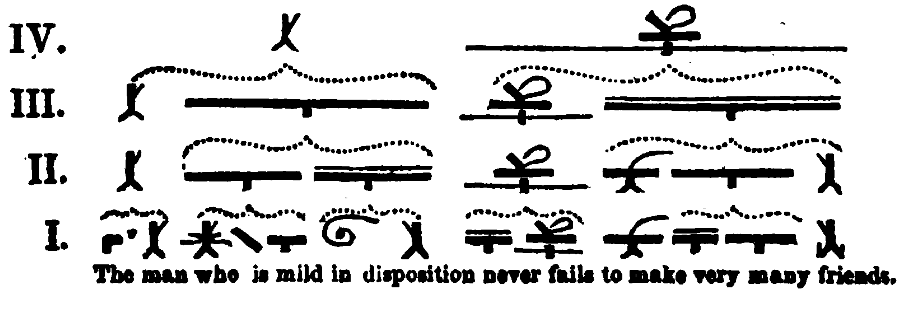
\includegraphics[width=\textwidth]{figures/vol1syntaxe2-img019.png}
    \caption{Diagramme de \citet{barnard1836analytic}}
    \small\textit{The man who is mild in disposition never fails to make very many friends.}
    ‘L’homme qui est doux de caractère n’échoue jamais à se faire de très nombreux amis.’
\end{figure}

    De la même façon, la relative \textit{who is mild in disposition} ‘qui est doux de caractère’ se comporte comme un adjectif (cf. le symbole 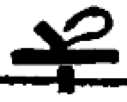
\includegraphics[height=1.25ex]{figures/vol1syntaxe2-img020.png} également associé à \textit{mild} ‘doux’ et \textit{many} ‘nombreux’) et sa combinaison avec \textit{the man} ‘l’homme’ se comporte comme un nom (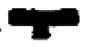
\includegraphics[height=1.25ex]{figures/vol1syntaxe2-img021.png}) ; de même, \textit{to make very many friends} ‘à se faire vraiment beaucoup d’amis’ se comporte comme un adverbe et sa combinaison avec \textit{never fails} ‘n’échoue jamais’ comme un verbe (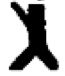
\includegraphics[height=1.25ex]{figures/vol1syntaxe2-img022.png}). Par contre Barnard ne considère pas la proposition comme équivalente au verbe et reste avec une structure sujet-prédicat pour la proposition que l’on retrouve de la grammaire de Port-Royal à la grammaire générative (voir l’encadré sur \textit{Fonctions syntaxiques et prédicat} du \chapfuturef{18}). Le diagramme qu’il propose peut néanmoins être considéré comme un premier exemple d’arbre de constituants et même d’arbre de constituants avec tête, puisque les étiquettes indiquent la catégorie de la tête comme en syntaxe X-barre (voir l’\encadref{sec:3.4.19} sur la \textit{Syntaxe X-barre}).

    Il semble que les contemporains de Barnard n’aient pas vraiment vu la portée de ces diagrammes et il faut attendre plus d’un siècle pour que, en \citeyear{nida1943morphology}, dix ans après la publication de \textit{Langage} de Bloomfield, Eugene Nida propose à nouveau des structures de constituants, dans une thèse intitulée \textit{A Synopsis of English Syntax}. Les structures proposées par Nida sont en fait des polygraphes (voir l’\encadref{sec:3.2.23} sur \textit{Graphe à bulles et polygraphe}) où chaque lien représente une connexion binaire et où les liens peuvent avoir pour sommet d’autres liens. Nida va ensuite enrichir son système, dans la republication de sa thèse en \citeyear{nida1966synopsys}, en ajoutant des symboles sur les liens (voir la figure \ref{fig:nida}) : les liens marquées d’une croix ($\times$)
    \todo[inline]{Verify that the size of the cross is equivalent to next figure}représentent une construction exocentrique, tandis que les liens marqués d’une flèche (~$\langle$ ou $\rangle$~) représentent une construction endocentrique, la flèche pointant vers la tête. Dans le diagramme ci-dessous, \textit{the} et \textit{men} sont connectés par un lien $\rangle$ indiquant que \textit{the} dépend de \textit{men}, puis \textit{by} est lié à ce lien par un lien $\times$ indiquant que la construction n’a pas de tête. Une telle représentation est équivalente à un arbre de constituants binaire (voir la \sectref{sec:3.4.21} sur \textit{Arbre de constituants binaires et polygraphe}).

    \begin{figure}[H]
        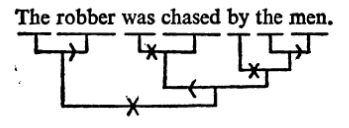
\includegraphics[width=\textwidth]{figures/vol1syntaxe2-img023.png}
        \caption{Représentation syntaxique de \citet{nida1966synopsys}}
        \label{fig:nida}
        \small\textit{The robber was chased by the men.} ‘Le voleur a été poursuivi par les hommes.’
    \end{figure}
         \todo[inline]{Reduce the figure to adapt the size of the font}
     
    Une représentation similaire a été proposée dans les années 1950 par Charles Hockett (voir son ouvrage \textit{A course in modern linguistics} de \citeyear{hockett1958course}). Cette représentation, connue aujourd’hui sous le nom de \textstyleTermesapprof{boîtes de Hockett} n’est pas un arbre (au sens où les branches ne sont pas explicites), mais plutôt un emboîtement de constituants, assez proche de l’arbre de dépendance avec projections intermédiaires de la figure \ref{fig:laponie-proj}. Dans le diagremme de la figure \ref{fig:hockett1}, les unités de bases sont les syntaxèmes (on notera la décomposition de la forme verbale \textit{wants} en \textit{want}{}-\,\textrm{${\oplus}$}{}\,-\textit{s}) et les intonèmes (les «~signes~» prosodiques) sont discrétisés (c’est-à-dire représentés par des symboles, ici 2, 3, 1 et ↓) et également intégrés à la décomposition. Il s’agit en fait d’une décomposition assez proche de la structure syntaxique X-barre qui ré-émergera 20 ans plus tard (voir l’\encadref{sec:3.4.19} sur la \textit{Syntaxe X-barre}), si ce n’est que Hockett considère encore que la combinaison \textit{sujet-verbe} est endocentrique. Le diagramme peut être enrichi de symboles \tikz [baseline=(node.base)] \node[draw,circle,inner sep=0pt] (node) {<}; ou \tikz [baseline=(node.base)] \node[draw,circle,inner sep=0pt] (node) {>}; indiquant, comme chez Nida, la dépendance (voir figure \ref{fig:hockett2}).

    \begin{figure}[H]
        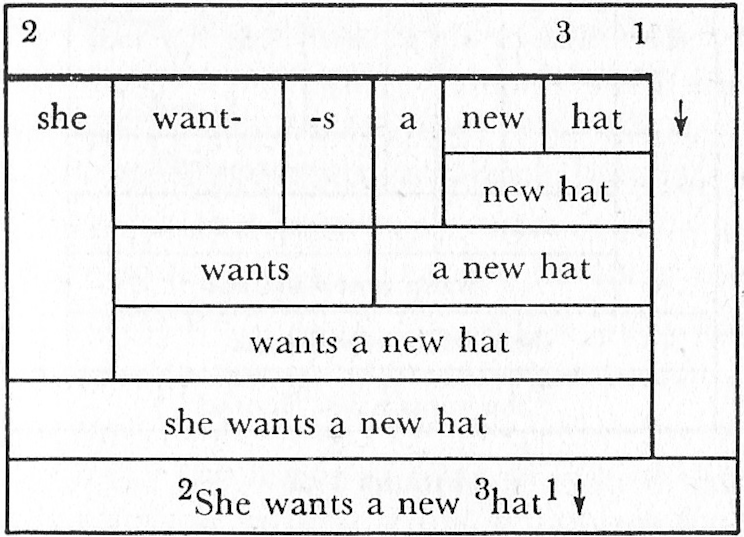
\includegraphics[width=7cm]{figures/vol1syntaxe2-img024.png}
        \caption{Boîtes de \citealt{hockett1958course}\label{fig:hockett1}}
        \textit{She wants a new hat.} ‘Elle veut un nouveau chapeau.’
    \end{figure}
        
    \begin{figure}[H]
        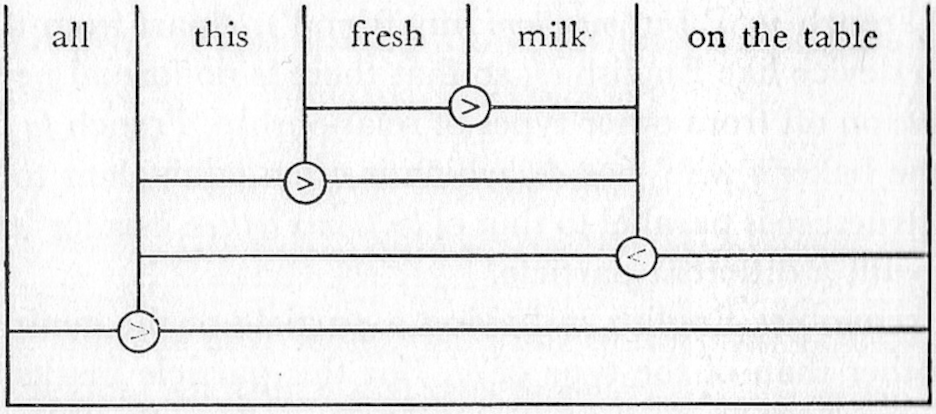
\includegraphics[width=10cm]{figures/vol1syntaxe2-img025.png}
        \caption{Boîtes de \citealt{hockett1958course} avec marquage des dépendances\label{fig:hockett2}}
        \textit{all this fresh milk on the table} ‘tout ce lait frais sur la table’
    \end{figure}

 
    Dans les représentations de Hockett, chaque module de trois cases (voir figure \ref{fig:hockett3}) est à lire comme une \hi{construction}, comme le remarque \citet{hockett1958course} (dans le chapitre \textit{Form classes and constructions}). Une telle analyse est contemporaine des grammaires de réécriture de Chomsky (voir l’\encadref{sec:3.5.30} sur la \textit{Grammaire de réécriture}) et son objectif est absolument similaire. On notera néanmoins que la représentation de Hockett met autant en avant la combinaison de A et B que la relation partie-tout de A ou de B avec le tout C qu’ils forment.

    \begin{figure}[H]
    \begin{subfigure}[t]{.5\textwidth}\centering
    \begin{tikzpicture}[every node/.style={font=\strut}]
    \node at (0,0) (A) {A};
    \node at (1,0) (B) {B};
    \node at (0.5,-1.25) (C) {C};
    \node [draw,fit =(A) (B) (C)] (box) {};
    \draw (box.east) -| (box.north)
          (box.west) -| (box.north);
    \node at (box.center) [draw,circle,fill=white,inner sep=-1pt] {<};
    \end{tikzpicture}
    \caption{Construction chez Hockett}
    \end{subfigure}\begin{subfigure}[t]{.5\textwidth}\centering
        \begin{tikzpicture}
        \node [CircleFillNode] (root) {}
            child { node [CircleFillNode] {} edge from parent node [midway,anchor=east] {T} }
            child { node [CircleFillNode] {} };
        \node [above=1pt of root] {C};
        \node [below=1pt of root-1] {A};
        \node [below=1pt of root-2] {B};
        \end{tikzpicture}
        \caption{Construction dans un arbre de constituants avec tête}
    \end{subfigure}
    \caption{{\color{red}Please provide a caption for the parent Figure.}\label{fig:hockett3}}
    \end{figure}   

    On attribue généralement l’introduction des arbres de constituants à Chomsky. On en trouve dans son article de \citeyear{chomsky1955three}, mais il est intéressant de noter que le diagramme en constituants introduit dans \textit{Syntactic Structures} de \citeyear{chomsky1957syntactic} n’est pas stricto sensu un arbre. Ce diagramme, donné dans la figure \ref{fig:chomsky57}, apparaît dans le chapitre 4 intitulé \textit{Phrase structure} ‘Structure syntagmatique’, où Chomsky introduit les règles de réécriture, comme \textit{Sentence → NP + VP}. Dans le diagramme, il n’y a pas, comme dans les arbres de constituants ordinaires, de relations partie-tout entre le nœud \textit{Sentence} et les constituants immédiats \textit{NP} et \textit{VP}. Au lieu de cela, il y a un lien entre \textit{NP} et \textit{VP} correspondant au symbole + de la règle et que l’on peut interpréter comme un lien de connexion, ainsi qu’un lien entre le nœud \textit{Sentence} et le lien de connexion correspondant à l’opération de réécriture représentée par le symbole \textit{→} dans la règle. Le diagramme est donc un polygraphe.

\begin{figure}[H]
%     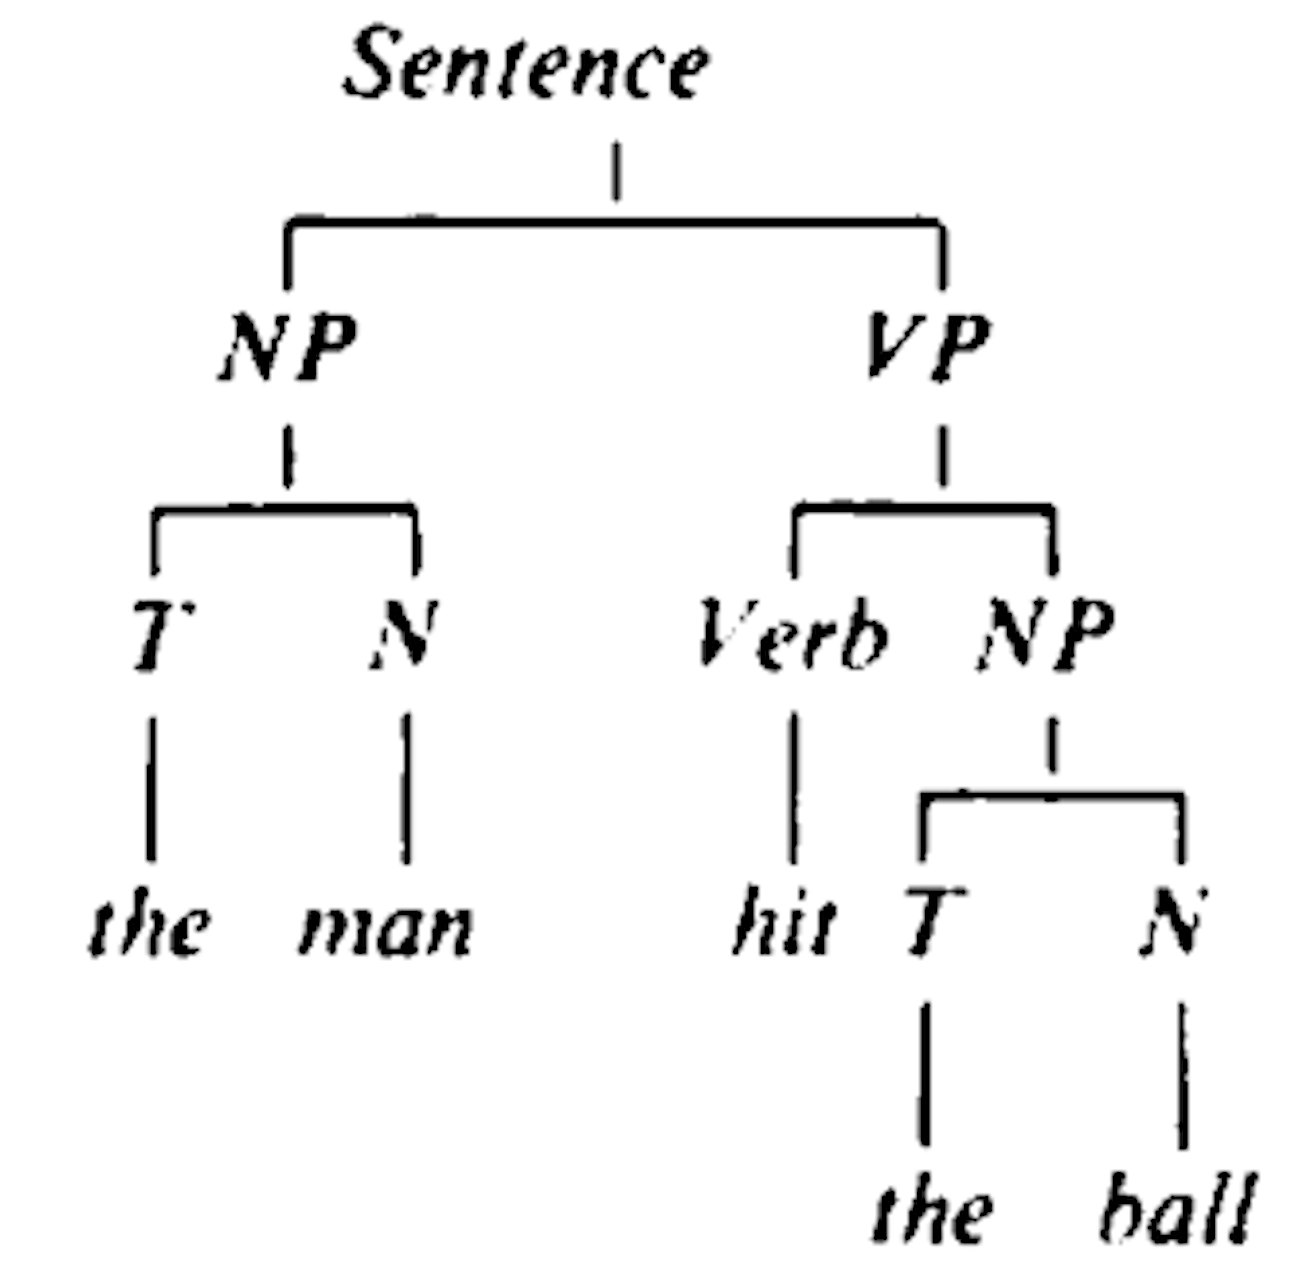
\includegraphics[width=\textwidth]{figures/vol1syntaxe2-img026.png}
    \begin{forest} forked edges, for tree = {font=\itshape}
    [Sentence
      [NP [T [the]]
          [N [man]]
      ]
      [VP [Verb [hit]]
          [NP [T [the]]
              [N [ball]]
          ]
      ]
    ]    
    \end{forest}
    \caption{Diagramme syntaxique (polygraphique) de \citet{chomsky1957syntactic}}
    \small\textit{The man hit the ball.} ‘L'homme frappa le ballon.’\label{fig:chomsky57}
\end{figure}

\begin{figure}[H]
% %     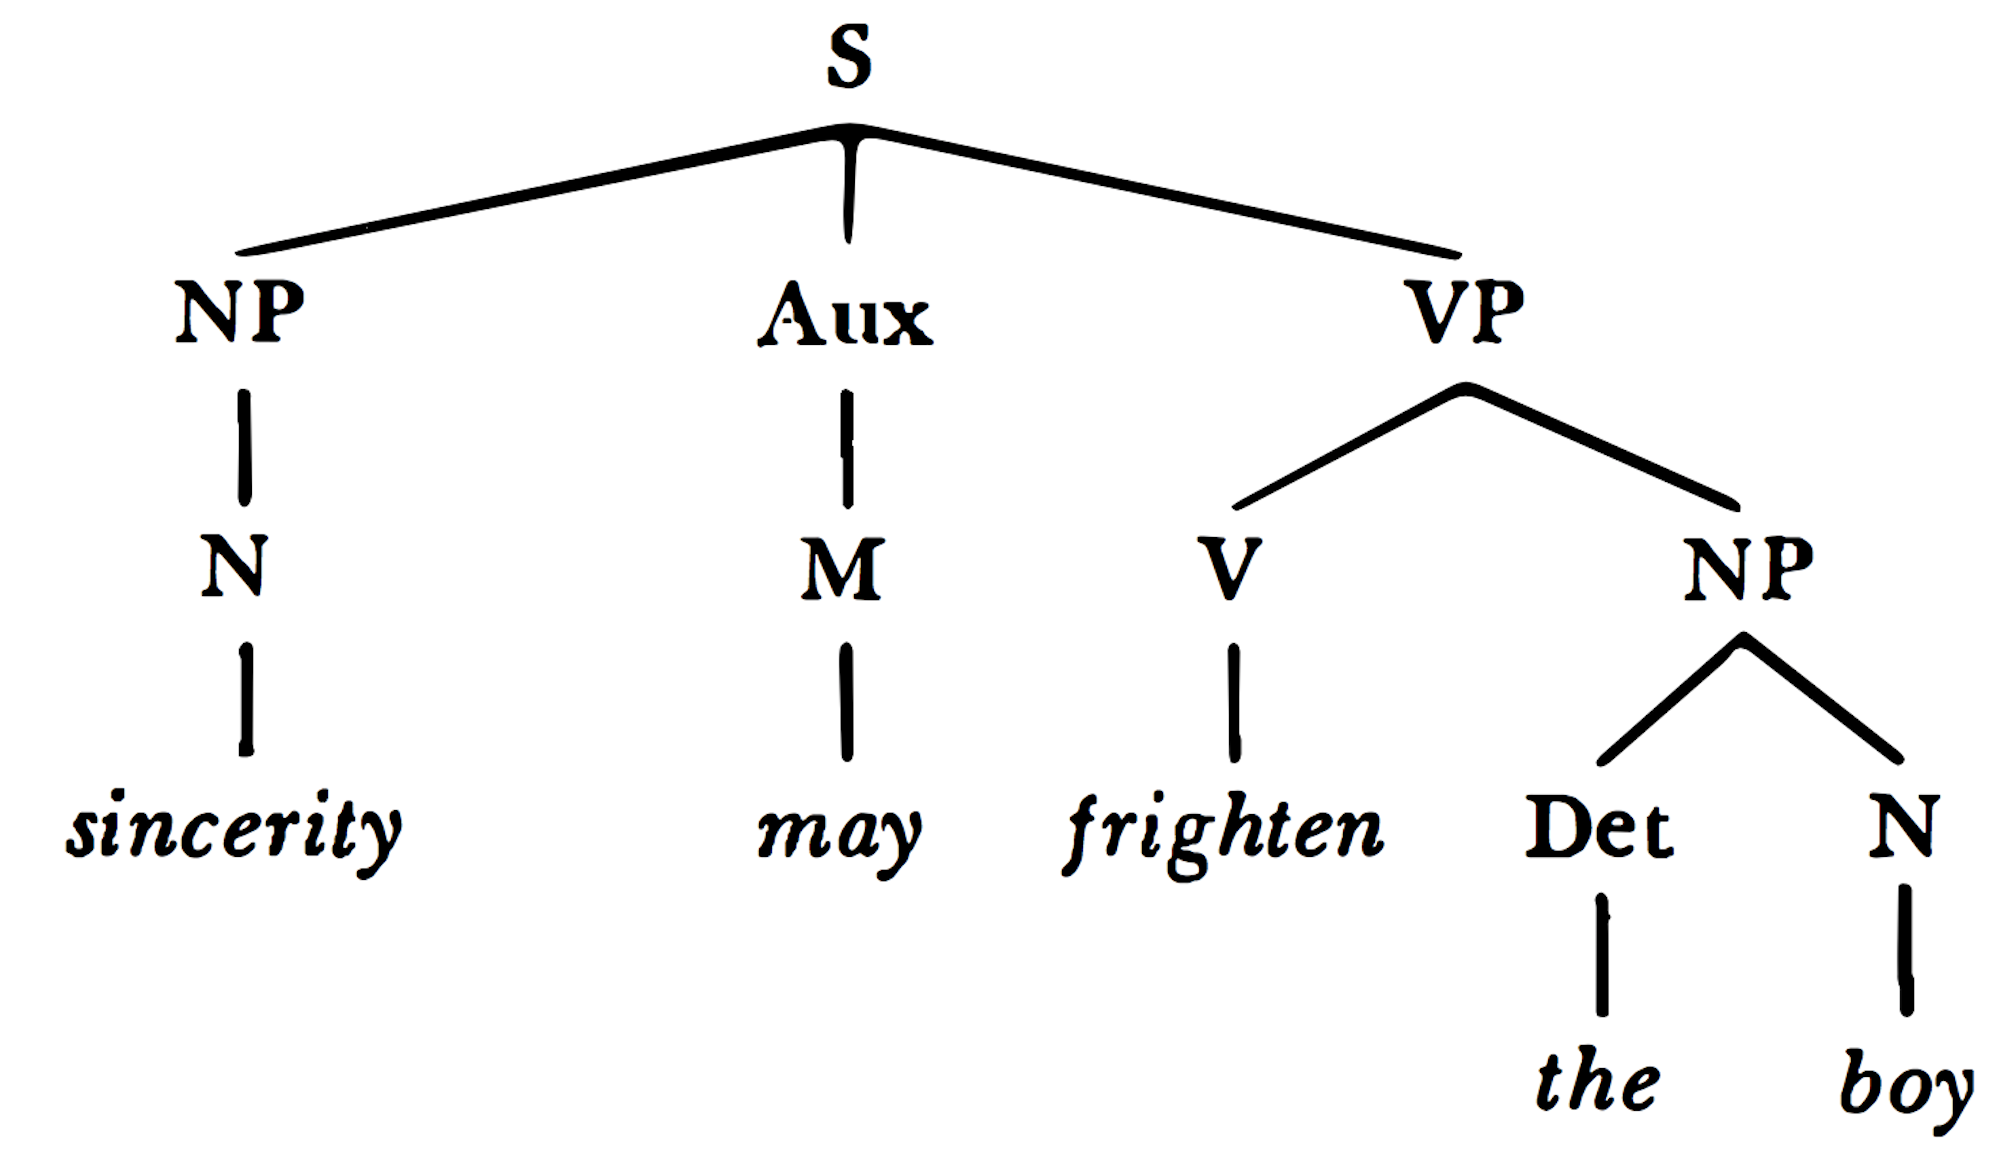
\includegraphics[width=\textwidth]{figures/vol1syntaxe2-img027.png}
   \begin{forest}
   [\normalfont S, calign=child, calign child=2
     [NP [N [\itshape sincerity]]]
     [Aux [M [\itshape may]]]
     [VP [V [\itshape frighten]]
         [NP [Det [\itshape the]]
             [N [\itshape boy]]
         ]
     ]
   ]
   \end{forest}
    \caption{Arbre syntaxique de \citet{chomsky1965aspects}\label{fig:chomsky65}}
   \small\textit{Sincerity may frighten the boy} ‘La sincérité peut effrayer le garçon’ 
\end{figure}

    Dans son deuxième livre, \textit{Aspects of the Theory of Syntax}, publié en \citeyear{chomsky1965aspects}, Chomsky revient à des arbres (voir un exemple dans la figure \ref{fig:chomsky65}). On notera que si le diagramme de 1957 est fondamentalement binaire, la binarité n’est plus exigée dans les arbres de 1965. Elle réapparaîtra dans les travaux suivants et notamment la syntaxe X-barre.
}
\loupe[sec:3.4.18]{Binarité, construction et connexion}{%
    L’exigence de \textstyleTermesapprof{binarité} des arbres de constituants est antérieure à l’usage de la représentation en arbre. L’idée qu’une décomposition représente une \textstyleTermesapprof{construction} élémentaire est déjà bien présente dans \textit{Language} de Leonard \citet{bloomfield1933language}. Bloomfield donne l’exemple de la construction \textit{actor-action}, que l’on pourrait appeler la construction \textit{subjectale}, pour reprendre un terme proposé par Igor \citet{melcuk1988dependency}. Autrement dit, il existe dans la phrase ordinaire une combinaison remarquable qui est celle du sujet avec le prédicat verbal (qu’on le conçoive comme le verbe seul ou comme un «~groupe verbal~», cela ne change rien pour nous, en termes de connexion). Cette construction (il s’agit bien d’une construction, au sens où on l’entend encore aujourd’hui, par exemple dans les \textstyleTermesapprof{Grammaires de constructions}) (voir les \textit{Lectures additionnelles}) est bien binaire, mettant en relation deux éléments, le sujet et le prédicat verbal. Selon les formalismes, cette construction sera représentée par une connexion ou une décomposition (voir la figure \ref{fig:subjectale}).

 \begin{figure}[H]
    \begin{minipage}[c]{.3\linewidth}\centering
      \begin{tikzpicture} 
        \node [CircleNode,label=below:N] at (0,0) (A) {};
        \node [CircleNode,label=below:V] at (2,0) (B) {};
        \draw[-{Triangle[]}] (B) to [bend right] node [midway,above,font=\itshape] {sujet} (A);
      \end{tikzpicture}
    \end{minipage}
    \begin{minipage}[c]{.3\linewidth}\centering
      \begin{forest}
       forked edges, for tree = {font=\normalfont}
       [S [NP] [VP]]
      \end{forest}
    \end{minipage}
    \begin{minipage}[c]{.3\linewidth}\centering
      \begin{forest} for tree = {font=\normalfont}
        [S [NP] [VP]]
      \end{forest}
    \end{minipage}    
    \caption{\label{fig:subjectale} Trois représentations de la construction subjectale}
 \end{figure}
    \todo[inline]{the second figure is not a forked edge. It is a vertical edge and a horizontal edge-brace separated by a small space (see figure \ref{fig:chomsky57})}

    Le premier diagramme de la figure \ref{fig:subjectale} dit qu’il y a une unité dont la tête est un nom (N) qui dépend d’un verbe (V) par une relation \textit{sujet}, le deuxième diagramme \citep{chomsky1957syntactic} dit qu’il y a un groupe nominal (NP, \textit{noun phrase}) et un groupe verbal (VP, \textit{verbal phrase}) qui se connecte pour former ensemble une phrase (S, \textit{sentence}), tandis que le troisième diagramme dit que la phrase S possède deux composantes, un NP et un VP. Même si cela n’apparaît pas au premier regard, il s’agit de trois représentations de la même construction. Qui plus est, ces trois descriptions sont moins éloignées qu’il n’y paraît à première vue : comme on l’a déjà vu dans le \chapref{sec:3.2} sur la \textit{Connexion} et comme on le verra à nouveau dans la \sectref{sec:3.4.21} sur \textit{Arbre de constituants binaires et polygraphes}, on passe de l’une à l’autre en réifiant ou déréifiant les relations partie-tout de la relation \textit{sujet}.

    L’exigence de binarité est une propriété partagée par de nombreuses analyses en constituants et par les analyses en dépendance : de la même façon que les constructions sont encodées, dans un arbre de dépendance, par des \hi{dépendances}, c’est-à-dire des \hi{relations liant deux à deux des mots}, les constructions seront encodées, dans un arbre de constituants binaire, par des \hi{décompositions binaires}, c’est-à-dire des \hi{combinaisons deux à deux de constituants}, .

    La principale différence dans les deux approches concerne la façon dont les différentes constructions sont repérées dans la structure. Dans le cadre de la syntaxe de dépendance, les constructions sont distinguées par l’étiquetage fonctionnel des dépendances (voir le \chapfuturef{18} sur les \textit{Relations syntaxiques}) et donc par une dénomination explicite de la construction : ainsi l’étiquette \textit{sujet} sur la dépendance plus haut indique qu’il s’agit de la construction subjectale. Dans le cadre de la syntaxe de constituants, les primitives sont les catégories et le repérage entre les constructions est fait par la configuration et les catégories : ainsi le sujet est le NP sous S, tandis que l’objet est le NP sous VP (voir la figure \ref{fig:objectale} qui compare les deux modes de représentation).

\begin{figure}[H]
  \begin{minipage}[c]{.3\linewidth}\centering
     \begin{forest} for tree = {font=\normalfont}
       [S [NP] [VP [V] [NP]]]
     \end{forest}
    \end{minipage}\hfill\begin{minipage}[c]{.6\linewidth}\centering
    \begin{tikzpicture}
      \node at (0,0) [CircleNode,label=below:N] (A) {};
      \node at (2,0) [CircleNode,label=below:V] (B) {};
      \node at (4,0) [CircleNode,label=below:N] (C) {};
      \path [-{Triangle[]}] (B) edge [bend right] node [midway,above,font=\itshape]
        {sujet} (A)
                                edge [bend left] node [midway,above,font=\itshape]
        {objet} (C);
    \end{tikzpicture}
    \end{minipage}
   \caption{\label{fig:objectale}Deux représentations des constructions subjectale et objectale}
\end{figure}
}
\loupe[sec:3.4.19]{Syntaxe X-barre}{%
    La \textstyleTermesapprof{Syntaxe X-barre} est la version la plus aboutie de l’\hi{analyse en constituants immédiats} (ACI) (voir la \sectref{sec:3.2.25} éponyme). Elle est développée à partir des années 1970 par Noam Chomsky et son étudiant Ray Jackendoff.

    L’innovation majeure de la Syntaxe X-barre est que \hi{tout constituant} est considéré comme étant la \hi{projection d’une} \hi{tête}. Dans les versions précédentes de l’ACI, la phrase était décomposée en un groupe substantival et un groupe verbal (cf. la fameuse règle S \textrm{→} NP VP), ce qui en faisait un constituant exocentrique. Le fait que tout constituant ait une tête rend la Syntaxe X-barre extrêmement proche d’une analyse en dépendance. (Seule la coordination est encore parfois traitée comme une construction symétrique dont les conjoints sont les co-têtes ; voir \encadref{sec:3.4.26} sur les \textit{Deux types d’arbres de constituants}.)

    La deuxième caractéristique de la Syntaxe X-barre est que les \hi{nœuds} \hi{de base} sont des \hi{syntaxèmes} et non des mots. Il y a donc deux types de constituants considérés, les \hi{projections lexicales}, dont la tête est un lexème, et les \hi{projections} dites \hi{fonctionnelles} dont la tête est un syntaxème flexionnel (une catégorie fonctionnelle dans les termes de la Syntaxe X-barre).

    La troisième caractéristique de la Syntaxe X-barre est que l’arbre de constituant est \hi{ordonné} et aucun constituant n’est discontinu, ce qui, pour les raisons que nous avons exposé dans l’\encadref{sec:3.2.7} \textit{De la non-séparation des ordres au mouvement}, entraîne la présence de nombreuses positions occupées par des traces co-indicés avec d’autres positions.

    La quatrième caractéristique de l’arbre X-barre est qu’il est \hi{binaire}. Ainsi la combinaison de chaque dépendant avec son gouverneur correspond à une décomposition binaire différente, ce qui, d’une certaine façon, rapproche encore plus cet arbre d’un arbre de dépendance (voir l’\encadref{sec:3.4.18}). La conséquence est que si un syntaxème a beaucoup de dépendants, il sera la tête d’autant de projections. Si le syntaxème est de catégorie X, sa \hi{projection maximale} est notée XP (\textit{X Phrase}) et ses \hi{projections intermédiaires} X’ (à l’origine elles étaient notées $\overline{\text{X}}$, avec une ou plusieurs barres au-dessus de X, d’où le nom de syntaxe X-barre).

    La Syntaxe X-barre considère de plus que l’élément sous XP a des propriétés différentes des éléments sous X’ : le premier est un \hi{spécifieur}, alors que les autres sont des \hi{compléments} (figure \ref{fig:Xbarre}). Dans certaines versions de la Syntaxe X-barre \citep{jackendoff1977x}, les ajouts (ou modifieurs) sont structurellement distingués des compléments actanciels par l’ajout d’un niveau de stratification supplémentaire dans la configuration de base (c’est-à-dire que XP porte une «~barre~» supplémentaire).

\begin{figure}[H]
    \begin{forest} for tree = {font=\normalfont}
    [XP,calign=child, calign primary child=2
        [spécifieur] [X', calign=child, calign primary child=1
            [X] [complément]
        ]
    ]
    \end{forest}
     \caption{Configuration de base de la Syntaxe X-barre}
    \label{fig:Xbarre}
\end{figure}

    En conclusion, l’arbre de constituants de la Syntaxe X-barre est assez différent des arbres de constituants plats. Les deux sont des \hi{arbres de constituants avec têtes}, mais le dernier ne contient que des projections maximales, qui, qui plus est, peuvent former des constituants discontinus. L’arbre X-barre ne repose pas vraiment sur des tests de constituance (qui, comme on l’a vu dans l'\encadref{sec:3.4.11}, caractérisent essentiellement les projections maximales), mais sur des \hi{principes configurationnels}. En d’autres termes, plus la géométrie d’un arbre permet de prédire de propriétés syntaxiques de l’énoncé qu’il représente, plus l’arbre a de raisons d’être. Ainsi, par exemple, le fait que le groupe substantival qui suit \textit{mange} possède des propriétés différentes dans les deux phrases suivantes devrait conduire à des configurations différentes, ce qui amène à compliquer à dessein la structure :

\ea
\ea   \textit{Pierre mange le pain.}
\ex   \textit{Pierre mange la nuit.} 
\z
\z

    Dans l’approche que nous développons ici, ces deux énoncés auront la même «~structure~» syntaxique (c’est-à-dire le même squelette structurel), mais les groupes substantivaux \textit{le pain} et \textit{la nuit} auront des fonctions totalement différentes (voir \chapfuturef{18} sur les \textit{Relations syntaxiques}).

    On peut s’étonner du fait que la syntaxe X-barre, dont l’objectif est de rendre compte des propriétés syntaxiques par des configurations géométriques, n’ait pas cherché à encoder structurellement une notion aussi fondamentale que la notion de \textit{tête}, ce que font pourtant assez simplement les structures de dépendance !
}
\loupe[sec:3.4.20]{Le groupe verbal}{%
    Le terme \textit{groupe verbal} (angl. \textit{verb phrase}, \textit{VP}) n’est pas utilisé de manière consistance dans la littérature. Ce terme désigne selon les auteurs deux notions différentes, que nous appellerons VP1 et VP2 :

    \begin{itemize}
    \item VP1 est une \hi{projection partielle} de la \hi{forme verbale} sans son sujet ;
    \item VP2 est la \hi{projection maximale} du \hi{lexème verbal}.
    \end{itemize}
    Les deux notions sont souvent confondues, alors qu’elles renvoient à des constituants différents (voir la figure \ref{fig:VP1VP2}) et à des cadres théoriques différents.

    VP2 est une notion théoriquement valable, mais qui suppose que l’on travaille avec la \hi{granularité des syntaxèmes}. Il y a alors lieu de considérer que le sujet dépend plutôt de la flexion (voir la \sectref{sec:3.2.18} \textit{Structures de connexion, granularité et critères}) et donc VP2 est la \hi{projection maximale du lexème verbal}, constituée du lexème verbal et de tous les éléments qu’il régit à l’exception du sujet. On notera néanmoins que VP2 n’est pas une unité autonomisable (puisque le lexème verbal n’apparaît jamais sans flexion) et qu’elle n’est donc qu’un objet théorique servant à expliciter, dans le cadre de l’analyse en constituants, que la réalisation du sujet est davantage liée à la nature de la flexion qu’à celle du lexème. Il y a, à notre avis, des moyens plus simples et plus directs, d’indiquer le lien entre le sujet et la désinence verbale.

    VP1 est une notion sans grand intérêt théorique de notre point de vue. Il s’agit d’un constituant intermédiaire (VP1 est le I’ de l’analyse de droite de la figure \ref{fig:theo-Xbarre}), qui résulte d’une stratification qui nous semble peu justifiée. En effet, rien ne permet de considérer que la forme verbale se combine d’abord avec ses autres dépendants avant de se combiner avec son sujet et donc de donner ainsi un statut spécial au sujet.

\begin{figure}[H]
\hfill
      \begin{multicols}{2}\raggedcolumns
    \begin{forest} for tree = {font=\normalfont}
     [S  [<\textit{sujet}>] [VP1 [\hspaceThis{VP1},roof]]]
    \end{forest}
    \hfill
    \begin{forest}
     [IP [<\textit{sujet}>] [I' [I [<\textit{flexion}>]] [VP2 [\hspaceThis{VP2},roof]]]]
    \end{forest}
    \end{multicols}\hfill
    \caption{\label{fig:VP1VP2}Configurations syntaxiques caractérisant respectivement VP1 et VP2}
\end{figure}

    Dernière remarque qui pourrait expliquer l’introduction de VP1 dans les analyses en constituants : l’anglais (qui est la langue la plus étudiée et la plus enseignée) a un \hi{constituant topologique} du type VP1 (voir les \textit{Exercices} du \chapref{sec:3.5}). Mais il est clair que la plupart des langues n’ont pas du tout cette configuration topologique et que, de toute façon, cela ne justifie pas l’introduction de VP1 dans la structure syntaxique au sens propre (que nous distinguons de la structure topologique).
}
\section{Arbre de constituants binaire et polygraphe}\label{sec:3.4.21}

Nous avons vu deux usages possibles de la représentation de la structure syntaxique par un arbre de constituants avec têtes : l’\hi{arbre de constituants plat} et l’\hi{arbre de constituants binaire}. (Nous confirmerons qu’il s’agit bien de deux usages différents du même formalisme dans l’\encadref{sec:3.4.25} sur \textit{Deux types d’arbres de constituants}, où nous montrons l’interprétation différente du branchement ternaire dans les deux conventions de représentation).

Nous avons vu que l’arbre de constituants plat pouvait être déduit trivialement (c’est-à-dire par un procédé de conversion automatique pure, sans ajout d’aucune information) d’un arbre de dépendance, ce qui n’est pas le cas de l’arbre de constituants binaire, qui nécessite d’ajouter un ordre de saillance sur les dépendances. Cela pourrait laisser penser que l’arbre de constituants plat est plus proche de l’arbre de dépendance : c’est vrai si on se place du point de vue formel, mais ça ne l’est pas si on se place du point de vue théorique. Comme on l’a vu dans l'\encadref{sec:3.4.15}, il y a derrière l’\hi{exigence de binarité}, le souci de dégager les différentes constructions syntaxiques, de les isoler les unes des autres. Et ce souci est commun avec les grammaires de dépendances. Nous allons montrer cela maintenant en repartant de l'exemple \ref{ex:laponie2} et de son arbre binaire le plus standard, donné dans la figure \ref{fig:laponie-T2}.

On peut interpréter chaque branchement binaire comme une connexion entre deux unités. Comme nous l’avons vu à la \sectref{sec:3.2.12} \textit{Représenter les combinaisons}, on peut représenter la combinaison A ${\oplus}$ B aussi bien par un lien entre A et B que par une bulle entourant A et B. Passer à un branchement binaire revient à \hi{réifier} les relations partie-tout entre A et B et l’unité qu’ils forment ensemble (voir l’\encadref{sec:3.4.22} qui suit pour des compléments sur la notion de réification). Ici nous proposons de faire l’inverse, c’est-à-dire de \hi{déréifier} les relations partie-tout qui constituent les branches d’un arbre de constituants. Comme, en plus, chaque branchement binaire indique une tête (la branche T), la déréification permet de récupérer une connexion orientée, c’est-à-dire une dépendance. Ceci est illustré dans la figure \ref{fig:dereification}.

\begin{figure}

\begin{tikzpicture}
  \node at (0,0) (A)  [CircleFillNode,label=below:A] {};
  \node at (2,0) (B)  [CircleFillNode,label=below:B] {};
  \node at (1,1) (U) [CircleFillNode,label=above:U] {};
  
  \draw (A) -- node [midway,anchor=base east] {T} (U)
            -- (B);

 \node at (3,0.5) {\huge$\Leftrightarrow$};
 \node at (4,0) (A2)  [CircleFillNode,label=below:A] {};
 \node at (6,0) (B2)  [CircleFillNode,label=below:B] {};
 \draw[-{Triangle[]}] (A2) to [bend left] node [midway,above] {U} (B2);
\end{tikzpicture}

\caption{\label{fig:dereification}Passage d’un branchement binaire à une dépendance par déréification d’un nœud non terminal}
\end{figure}

Si l’on applique la déréfication à tous les nœuds intérieurs de l’arbre de constituants binaire de la figure \ref{fig:laponie-T2}, on obtient la structure de la figure \ref{fig:polygraphe-ordre}. Cette structure est un \textstyleTermes{polygraphe} (voir définition formelle dans l’\encadref{sec:3.2.23} sur \textit{Graphe à bulles et polygraphe}) : ce n’est pas exactement un graphe, puisqu’un arc ne lie pas forcément deux nœuds (les nœuds sont les mots), mais il peut lier d’autres arcs entre eux ou un arc et un nœud. De plus, ce polygraphe est \textstyleTermes{orienté}, puisque chaque arc du graphe lie un gouverneur à un dépendant. Enfin ce polygraphe est implicitement \textstyleTermes{ordonné}, dans le sens où les nœuds du polygraphe sont disposés selon un ordre linéaire (celui des mots dans la phrase). De telles structures ont été proposées par le linguiste américain Eugene Nida dans sa thèse soutenue en \citeyear{nida1943morphology} (voir l’\encadref{sec:3.4.17} sur l’\textit{Historique des représentations syntaxiques par des diagrammes en constituants}.)

\begin{figure}
\caption{\label{fig:polygraphe-ordre}Polygraphe orienté et ordonné}
\begin{forest} for tree = {edge={draw=none},font=\itshape, fit=band}
[
 [ [beaucoup] [ [de] [gens] ] ]
 [ [aimeraient]
        [ 
          [ [passer] [Noël] ] 
          [ [en] [Laponie] ] 
        ] 
  ]
]
\begin{scope}[>={Triangle[]},overlay]
\draw[<-] (!2.north) +(0,.25) to [bend right,in=270,out=270] (!1.north) to (!1.south);
\draw[->] (!11.north)   to [bend left,out=90,in=90]   (!12.north) to (!12.south);
\draw[->] (!121.north)  to [bend left,out=90,in=90]                  (!122.north);
\draw[->] (!21.north)   to [bend left,out=90,in=90]                  (!22.north) to (!22.south);
\draw[->] (!221.south)  to [bend left,out=90,in=90]                  (!222.south);
\draw[->] (!2211.north) to [bend left,out=90,in=90]                  (!2212.north);
\draw[->] (!2221.north) to [bend left,out=90,in=90]                  (!2222.north);
\end{scope}
\end{forest}
\end{figure}
\todo[inline]{some arcs are different. It would be nicer if all the arcs were identical (with different sizes). The spaces between the head of the arrows and the dependent is irregular too.}


\maths[sec:3.4.22]{Réification et transitivité}{%
    Nous appelons \textstyleTermes{réification}, du latin \textit{res} ‘chose’, l'opération qui consiste à rendre concret un élément virtuel d'une structure, comme un point de contact entre deux objets. Pour mieux comprendre ce qu'est la réification, donnons un autre exemple, emprunté à la représentation sémantique des constructions transitives. Considérons une phrase élémentaire telle que :

    \ea\label{ex:frappe}
    \textit{Marie frappe Pierre.}
    \z
 Il y a là ce qu’on appelle un verbe transitif, \textit{frappe}, qui exprime une action d’un élément (\textit{Marie}) sur un autre (\textit{Pierre}). On dira encore que \textit{Marie} est l’\hi{agent} de l’action et \textit{Pierre} le \hi{patient}. Il y a alors plusieurs façons de représenter graphiquement le «~sens~» de cette phrase. Nous en proposons trois dans la figure \ref{fig:frappe-reif}.

% \begin{figure}[H]
   \ea
    \ea\attop{%
      \begin{tikzpicture}
        \node at (0,0) [ConcSet] (Marie) {Marie};
        \node [right=1mm of Marie, draw, signal, signal to=east, font=\itshape] (frappe) {frappe}; 
        \node [right=1mm of frappe, ConcSet] (Pierre) {Pierre};
      \end{tikzpicture}}\medskip\\
      \ex\attop{\begin{tikzpicture}
        \node at (0,0) [ConcSet] (frappe) {frappe};
        \node at (-2,-2) [ConcSet] (Marie) {Marie};
        \node at (2,-2) [ConcSet] (Pierre) {Pierre};
        \draw[-{Triangle[]}] (frappe) -- (Marie)  node [midway,left] {agent};
        \draw[-{Triangle[]}] (frappe) -- (Pierre) node [midway,right] {patient};
      \end{tikzpicture}}\medskip\\
      \ex\attop{\begin{tikzpicture}
        \node at (0,0) [ConcSet] (frappe) {frappe};
        \node at (-2,-4) [ConcSet] (Marie) {Marie};
        \node at (2,-4) [ConcSet] (Pierre) {Pierre};
        \node at (-2,-2) [draw,rectangle] (agent) {agent};
        \node at (2,-2) [draw,rectangle] (patient) {patient};
        \draw[-{Triangle[]}] (agent) edge node[midway,left] {2} (frappe)
                                     edge node[midway,left] {1} (Marie);
        \draw[-{Triangle[]}] (patient) edge node[midway,right] {2} (frappe)
                                     edge node[midway,right] {1} (Pierre);
      \end{tikzpicture}}
  \z
\z
% \todo[inline]{in the first diagram, we want to have 3 objects with the label inside. So frappe should inside the arrow and the arrow must have a unique outline (no line between the head and the body). See original. This a very special arrow that is unique in the book.}
% \todo[inline]{Make a figure and maintain a,b,c, please}
%   \caption{\label{fig:frappe-reif}Trois niveaux de réification pour la représentation du sens de \REF{ex:frappe}}
% \end{figure}

    Dans la représentation a, \textit{frappe} est directement modélisé comme une action de Marie sur Pierre : \textit{frappe} (\textit{Marie}, \textit{Pierre}). Dans la représentation b, les relations qui lient \textit{frappe} à \textit{Marie} et \textit{Pierre} sont explicitées et nommées \textit{agent} et \textit{patient}. Dans la représentation c, les relations agent et patient sont vues comme des objets à part entière reliant les mots de la phrase : agent~(\textit{Marie}, \textit{frappe}) + patient~(\textit{Pierre}, \textit{frappe}). On l’aura deviné, les trois représentations sont des réifications successives des relations d’une même structure.

    Si toute structure peut-être réifiée à l’infini, comment choisir le bon niveau de réification ? Faire de la relation entre deux objets un objet n’a d’intérêt que si l’on veut considérer cet objet en tant que tel et lui attribuer des propriétés. Dans le cas de la transitivité, on peut préférer la représentation b qui explicite les relations d’agent et de patient et permet donc d’en parler, par exemple pour décrire la voix passive (voir le \chapfuturefici{13}).

    Dans le cas de la relation de connexion, nous pensons qu’il n’est pas nécessaire d’expliciter les relations partie-tout que la connexion entretient avec les unités qu’elle connecte, d'autant que la connexion est pour nous une classe d'équivalence de combinaisons qui mettent en jeu des unités de granularité variée (voir la \sectref{sec:3.2.14} sur \textit{La connexion et ses instances}).}

\section{Polygraphe orienté et arbre de dépendance}\label{sec:3.4.23}

Si l’on s’abstrait complètement de l’ordre linéaire et que l’on garde uniquement le polygraphe orienté, on peut adopter la représentation de la figure \ref{fig:laponie-polygraphe-pur}, où chaque arc est représenté par une ligne droite avec le gouverneur au-dessus de son dépendant.

\begin{figure}
\caption{\label{fig:laponie-polygraphe-pur}Polygraphe orienté (non ordonné)}
\begin{turn}{-45}
	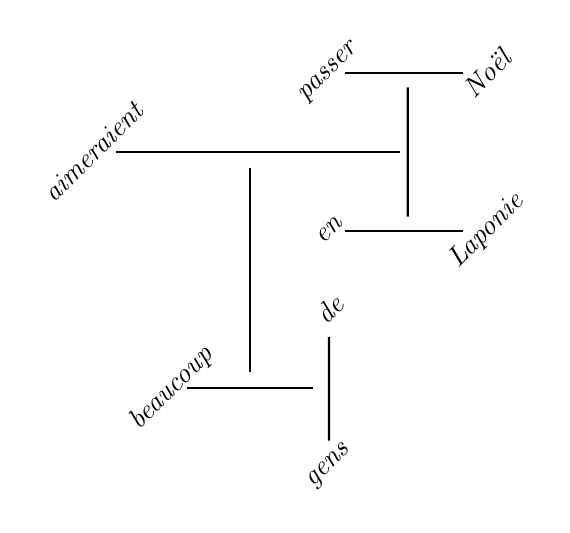
\begin{tikzpicture}\itshape
		\node (passer)   at (4,5)  [rotate=45] {passer};
		\node (b)   at (5,5)  [rotate=45] {};
		\node (Noël)   at (6,5)  [rotate=45] {Noël};
		%
		\node (aimeraient)   at (1,4)  [rotate=45] {aimeraient};
		\node (x)   at (3,4)  [rotate=45] {};
		\node (y)   at (5,4)  [rotate=45] {};
		%
		\node (en)   at (4,3)  [rotate=45] {en};
		\node (a)   at (5,3)  [rotate=45] {};
		\node (Laponie)   at (6,3)  [rotate=45] {Laponie};
		%
		\node (de)   at (4,2)  [rotate=45] {de};
		%
		\node (beaucoup)   at (2,1)  [rotate=45] {beaucoup};
		\node (z)   at (3,1)  [rotate=45] {};
		\node (c)   at (4,1)  [rotate=45] {};
		
		%
		\node (gens)   at (4,0)   [rotate=45]  {gens};
		%
		\draw[thick,shorten <=2mm, shorten >=3mm] (4,5) -- (6,5);
		\draw[thick,shorten <=3mm, shorten >=1mm] (1,4) -- (5,4);
		\draw[thick,shorten <=2mm, shorten >=3mm] (4,3) -- (6,3);
		% 2
		\draw[thick,shorten <=2mm, shorten >=2mm] (2,1) -- (4,1);
		
		%
		% \draw[thick] (z) -- (x);
		\draw[thick,shorten <=2mm, shorten >=2mm] (3,1) -- (3,4);
		\draw[thick] (gens) -- (de);
		\draw[thick] (a) -- (b);
	\end{tikzpicture}
\end{turn}
\todo[inline]{Nice figure! Just suppress the space around the figure}
\end{figure}

Bien que cela n’apparaisse pas au premier coup d’œil, cette structure est un extrait de la structure de la figure \ref{fig:laponie-polygraphe-ordre} : c’est le même \hi{polygraphe orienté} que précédemment, mais sans l’ordre des mots et avec une autre convention de représentation. Au lieu d’indiquer la hiérarchisation de la connexion par une flèche, celle-ci est indiquée en plaçant le gouverneur au-dessus du dépendant. Or ce polygraphe orienté, qui a donc été extrait automatiquement de l’arbre de constituants binaires en mettant en évidence les connexions, est très proche d’un arbre de dépendance. Pour obtenir l’arbre de dépendance, il suffit de \hi{faire glisser chaque dépendance} le long des dépendances sur lesquelles elle s’appuie, comme montré dans la figure \ref{fig:glissade}. Nous retombons ainsi sur l'arbre de dépendance de départ (voir figure \ref{fig:laponie-dep2}).

\begin{figure}
\begin{minipage}{.45\textwidth}\centering
\begin{forest}
nice empty nodes,for tree={font=\itshape}
[aimeraient
  [
    [ [en] [Laponie] ]
    [ [passer] [Noël] ]
  ]
]
\draw[-{Triangle[]}] (!111.south) -- (!112.south);
\draw[-{Triangle[]}] (!121.south) -- (!122.south);
\draw[-{Triangle[]}] (!12.west) +(-.5,0) -- ($(!11.east) +(.5,0)$);
\end{forest}
\end{minipage}\hfill%
\begin{minipage}{.05\textwidth}\centering
$\Rightarrow$
\end{minipage}\hfill%
\begin{minipage}{.45\textwidth}\centering
\begin{forest}
nice empty nodes,for tree={font=\itshape}
[aimeraient
  [passer
    [Noël]
    [en [Laponie] ]
  ]
]
\end{forest}
\end{minipage}
\caption{\label{fig:glissade}Passage du polygraphe orienté à un arbre de dépendance par «~glissade~»}
\todo[inline]{The figure must be completely reshaped. See original. The left part is a subpart of the previous polygraph. The right part must be in the same style, with the same edges. The three arrows in the left part indicate a sliding movement. They must be different from the arrow used for the dependency or the conversion. The arrow in the middle is a conversion arrow (big \textbackslash Rightarrow).}
\end{figure}



Nous appellerons \textstyleTermes{méthode par déréification }la méthode que nous venons de présenter, qui permet de passer d’un arbre de constituants binaire avec têtes à un arbre de dépendance. La méthode par déréification peut s’appliquer à des arbres de constituants dont certains branchements décrivent des constructions exocentriques et n’ont donc pas de marquage de la tête. Dans l’exemple \textit{le petit chien dort} (déjà étudié dans la \sectref{sec:3.3.23} \textit{Nom ou déterminant comme tête} ?), si l'on ne décide pas qui de l’article \textit{le} ou du nom \textit{chien} est la tête du groupe substantival, on obtient par déréification une connexion non orientée, qu’on ne peut pas faire «~glisser~» comme on l’a fait précédemment pour les connexions orientées. Comme le montre la figure \ref{fig:lechien2}, nous retombons sur le polygraphe de la figure \ref{fig:lechien}, que nous avions proposé pour l'analyse d'une construction exocentrique.

\begin{figure}
\begin{minipage}[c]{.45\textwidth}\centering
\begin{tikzpicture}[every node/.style={font=\strut}]
    \begin{scope}[
    every node/.style={CircleFillNode},
    sibling distance=15mm,
    level distance=2\baselineskip
    ]
        \node (root) {}
            child { node { } 
                    child { node { } }
                    child { node { } 
                        child { node { } }
                        child { node { } edge from parent node [reset shape, midway,anchor=base west] {T} }
                    }
                   }
            child { node { } edge from parent node [reset shape, midway, anchor=base west] {T} };
    \end{scope}
    \begin{scope}[every node/.style={font=\strut\itshape}]
    \foreach \pos/\text in {1-1/le, 1-2-1/petit, 1-2-2/chien, 2/dort} 
      {\node [below=1pt of root-\pos] {\text};}
    \end{scope}
    \end{tikzpicture}
    \end{minipage}
    \hfill%
      \begin{minipage}[c]{.05\textwidth}\centering
        \huge$\Rightarrow$
      \end{minipage}
    \hfill%
    \begin{minipage}[c]{.33\textwidth}\centering
    \begin{forest} for tree={font=\itshape}
    [dort
      [,nice empty nodes
        [le] [chien [petit]]
      ]
    ]
    \end{forest}
    \end{minipage}\hfill
\caption{\label{fig:lechien2}Conversion d'un arbre de constituants avec marquage partiel des têtes en une structure de dépendance par la méthode de déréification}
\end{figure}
\todo[inline]{the subfigure on the right is a polygraph with an horizontal line between le and chien, see figure \ref{fig:lechien}}

\section{Comparaison des méthodes par décomposition}\label{sec:3.4.24}

Nous avons présenté deux \hi{méthodes par décomposition} pour passer d’un arbre de constituants à un arbre de dépendance : la méthode de Lecerf ou méthode par agrégation des projections d’une part et la méthode par déréification d’autre part.

Les deux méthodes sont différentes et s’appliquent à des types d’arbres de constituants différents : la \hi{méthode de Lecerf} s’applique uniquement à des arbres de constituants avec têtes, puisqu’elle repose crucialement sur l’agrégation des projections d’une même \hi{tête~}; la \hi{méthode par déréification} s’applique à n’importe quel type d’arbre de constituants, mais elle ne donne des \hi{connexions binaires} que si elle est appliquée à un arbre binaire (voir l’\encadref{sec:3.4.26} pour le cas des branchements ternaires).

Néanmoins lorsque les deux méthodes sont appliquées à un arbre de constituants \hi{binaire avec têtes}, elles donnent le \hi{même arbre de dépendance} (voir \textit{Exercices}).

\section{Équivalences entre structures}\label{sec:3.4.25}

Nous avons présenté un grand nombre de structures plus ou moins équivalentes. La figure \ref{fig:rosace} rassemble ces différentes structures.

La partie droite de la figure montre le passage d’un arbre de dépendance à \hi{un arbre de constituants plat}, puis retour à l’arbre de dépendance, tandis que la partie gauche montre le passage d’un arbre de dépendance à un \hi{arbre de constituants binaire avec têtes}, puis retour à l’arbre de dépendance.

\begin{figure}
\caption{\label{fig:rosace}Équivalence entre les différentes représentations de la structure syntaxique de \REF{ex:laponie2}}
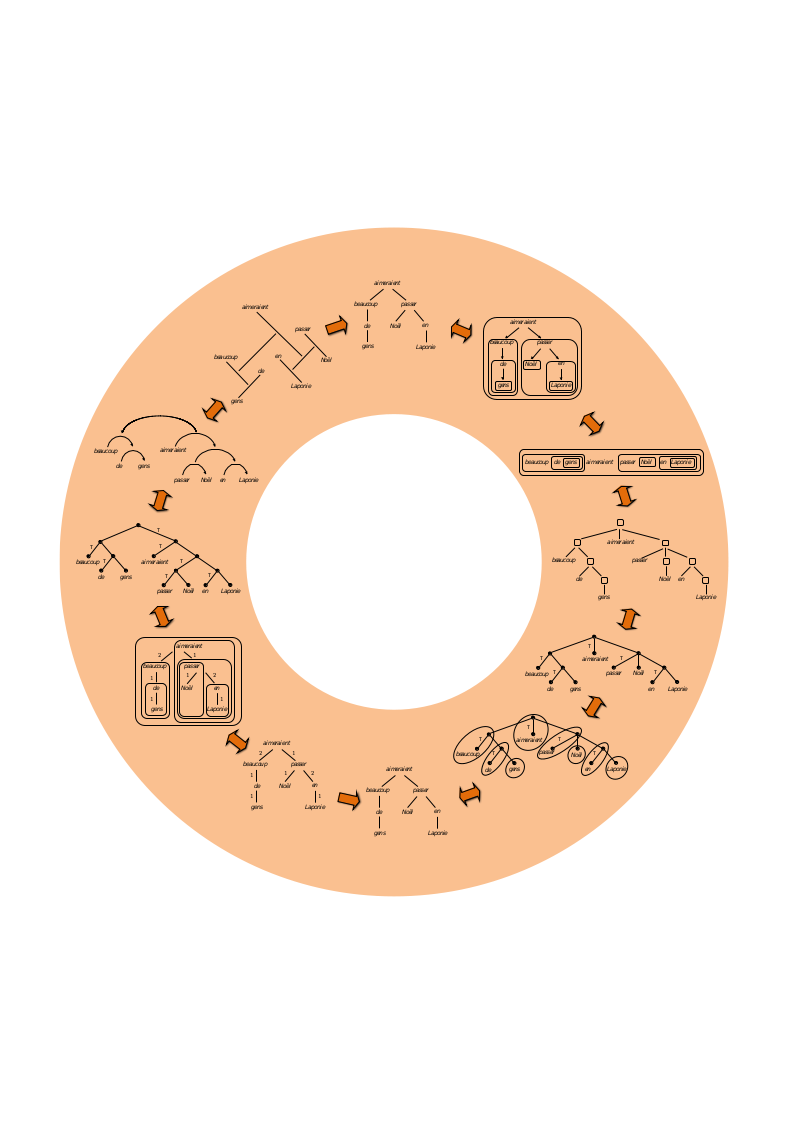
\includegraphics[width=\textwidth]{figures/vol1syntaxe2-img028.png}
\todo[inline]{This figure gather all the figures of the chapter. The arrows must be conversion arrows. I understand that is will be a lot of work to draw this figure, but it is the grand finale of the chapter and also of the book. When the figure is ready we could add it on the web page. And put is also at the begining of the book.}
\end{figure}

Chaque flèche $\Rightarrow$ ou $\Leftrightarrow$ entre deux structures symbolise une opération de conversion élémentaire permettant de passer d’une structure à une autre. Dans la plupart des cas, l’opération ne nécessite l’ajout d’aucune information et les deux structures sont équivalentes (nous ne considérons pas l’ordre linéaire sur les mots qui est des fois présent dans la structure et d’autres fois non). C’est le cas dans toute la partie droite de la figure, où toutes les structures sont équivalentes entre elles. Il s'agit de \hi{structures de constituants plates}. De la même façon, toutes les structures de la partie gauche sont équivalentes entre elles. Il s'agit de \hi{structures de constituants binaires avec têtes}. Elles contiennent une information supplémentaire qui est la stratification. Cette stratification, qui permet de stratifier les branchements non binaires, est indiquée dans la partie basse de la figure par l’ajout de l’ordre de saillance, lequel disparaît dans la partie haute, lorsque les «~glissades~» sont effectuées sur le polygraphe et qu’on revient à l’arbre de dépendance.

\loupe[sec:3.4.26]{Deux types d’arbres de constituants}{%
    Nous avons présenté dans ce chapitre deux types d’arbres de constituants avec têtes : les arbres de constituants plats et les arbres de constituants binaires comme ceux de la syntaxe X-barre. On peut penser que tout arbre de constituants plat peut être «~binarisé~» en introduisant des constituants intermédiaires. En fait, la différence est plus profonde et il s’agit à notre avis de deux façons assez différentes d’utiliser le même formalisme. La différence apparaît lorsqu’on regarde les branchements ternaires.

    Dans un arbre plat, les branchements ternaires sont courants. Ils apparaissent dès qu’un mot a au moins deux dépendants. Reprenons l’exemple de \textit{passer Noël en Laponie}, qui se décompose en trois morceaux, une tête (\textit{passer}) et ses deux dépendants (\textit{Noël} et \textit{en Laponie}) (voir la \sectref{sec:3.4.4} sur les \textit{Arbres de constituants avec têtes}).

\begin{figure}[H]
    \begin{minipage}[c]{.45\linewidth}\centering
    \begin{tikzpicture}[every node/.style={font=\strut}]
    \begin{scope}[
    every node/.style={CircleFillNode},
    sibling distance=15mm,
    level distance=2\baselineskip
    ]
        \node (root) {}
            child { node { } edge from parent node [reset shape, midway,anchor=base east] {T} } 
            child { node { } }
            child { node { } 
                child { node { } edge from parent node [reset shape, midway,anchor=base east] {T} }
                child { node { } }
                };
    \end{scope}
    \begin{scope}[every node/.style={font=\strut\itshape}]
    \foreach \pos/\text in {1/passer, 2/Noël, 3-1/en, 3-2/Laponie} 
      {\node [below=1pt of root-\pos] {\text};}
    \end{scope}
    \end{tikzpicture}
    \end{minipage}%
    \begin{minipage}[c]{.1\textwidth}\centering
    \huge$\Leftrightarrow$
    \end{minipage}%
    \begin{minipage}[c]{.45\textwidth}\centering
    \begin{forest} for tree={font=\itshape}
    [passer
      [Noël]
      [en [Laponie]]
    ]
    \end{forest}
    \end{minipage}
 \caption{\label{fig:laponie-ternaire}Branchement ternaire et correspondance par la méthode de Lecerf}
\end{figure}

    En appliquant la méthode de Lecerf à l’arbre plat à gauche de la figure \ref{fig:laponie-ternaire}, on obtient l’arbre de dépendance à droite. Comme on le voit, le branchement ternaire est interprété comme deux connexions binaires, la connexion entre \textit{passer} et \textit{Noël} et la connexion entre \textit{passer} et \textit{en Laponie}.

    Dans un arbre binaire, il en va tout autrement, puisque, comme nous l’avons montré ci-dessus (\sectref{sec:3.4.21} sur \textit{Arbres de constituants binaire et polygraphe}), \hi{chaque branchement correspond à une unique connexion}. Si un tel arbre contient un branchement ternaire, il doit être interprété comme une \hi{connexion ternaire} (voir l’\encadref{sec:3.2.17} éponyme). La syntaxe X-barre, qui revendique l’usage des arbres binaires, s’est aventurée à proposer des branchements ternaires pour la coordination (notamment dans l'ouvrage de \citealt{jackendoff1977x}). On trouve déjà les mêmes arbres dans \citealt{hockett1958course} ; la figure \ref{fig:hockett-coord} les boîtes de Hockett pour la coordination où le branchement est ternaire et symétrique, avec une position bien différenciée pour la conjonction).

\begin{figure}[H]
%     \includegraphics{}
    \caption{\label{fig:hockett-coord}Branchement ternaire dans une boîte de Hockett}
     \todo[inline]{Structure of this graph could not be obtained from the original submission file}
    \todo[inline]{I drew it. Is it possible to draw it again?}
\end{figure}


    Cette analyse est ce qu’on appelle l’\hi{analyse symétrique de la coordination} (voir le \chapfuturef{19}) : dans \textit{Marie et Pierre dorment}, les conjoints (c’est le nom que l’on donne aux éléments coordonnés, \textit{Marie} et \textit{Pierre}) sont considérés comme des co-têtes, qui contribuent à égalité à la distribution du syntagme (lequel déclenche un accord pluriel du verbe). Il s’agit alors d’une construction ternaire, que nous pouvons représenter par une connexion ternaire en suivant les conventions de représentation utilisées par Tesnière dans son article de \citeyear{tesniere1934comment} \textit{Comment construire une syntaxe ?} : les deux conjoints \textit{Marie} et \textit{Pierre} sont au même niveau, reliés par une connexion horizontale, et la conjonction, qui est le troisième «~sommet~» de cette connexion, est placé en dessous.

\begin{figure}[H]
    \begin{minipage}[c]{.55\linewidth}\centering
    \begin{tikzpicture}[every node/.style={font=\strut}]
    \begin{scope}[
    every node/.style={CircleFillNode},
    level 1/.style={sibling distance=30mm},
    level 2/.style={sibling distance=15mm},
    level distance=2\baselineskip
    ]
        \node (root) {}
            child { node { } 
                child { node { } edge from parent node [reset shape, midway, anchor=base east] {T} }
                child { node { } }
                child { node { } edge from parent node [reset shape, midway, anchor=base west] {T} }
                  }
            child { node { } edge from parent node [reset shape, midway, anchor=base west] {T} }; 
    \end{scope}
    \begin{scope}[every node/.style={font=\strut\itshape}]
    \foreach \pos/\text in {1-1/Marie, 1-2/et, 1-3/Pierre, 2/dorment} 
      {\node [below=1pt of root-\pos] {\text};}
    \end{scope}
    \end{tikzpicture}
    \end{minipage}%
    \begin{minipage}[c]{.1\linewidth}\centering\huge$\Rightarrow$\end{minipage}%
    \begin{minipage}[c]{.35\textwidth}\centering
    \begin{forest} for tree={font=\itshape}
    [dorment
      [,nice empty nodes
        [Marie] [Pierre]
      ] 
    ]
    \node at (.25,-1) {\itshape et};
    \end{forest}
    \end{minipage}
    \caption{\label{fig:polygraphe-coord}Branchement ternaire et correspondance par la méthode de déréification}
\end{figure}
\todo[inline]{The right figure is a polygraph. The word "et" is a label on the horizontal edge. See original}

    La structure de dépendance de droite peut être obtenue en appliquant la méthode de conversion par déréification à l’arbre de constituant à gauche. Le branchement ternaire donne une connexion ternaire, où \textit{Marie} et \textit{Pierre} occupent des positions symétriques (puisqu’ils sont co-têtes), tandis que la conjonction \textit{et} occupe une troisième position, comme «~dépendant~» des co-têtes. La convention de Tesnière rend bien compte de cela.

    En conclusion, on note que \hi{le formalisme des arbres de constituants est ambigu~}: il ne permet pas de distinguer une analyse plate (on ne souhaite pas considérer de constituants intermédiaires) et une connexion ternaire (on souhaite indiquer que les éléments ne se combinent pas toujours deux à deux, mais parfois par trois). Celui des structures de dépendance le permet, à condition de considérer des structures qui ne sont plus entièrement hiérarchisées et qui contiennent des connexions ternaires.
}
\section{Combiner les méthodes ascendante et descendante}\label{sec:3.4.27}

A l’issu de ce chapitre et des deux précédents, nous avons présenté plusieurs méthodes pour construire la structure syntaxique. Nous aimerions conclure ce chapitre en montrant comment combiner les méthodes ascendante (par combinaison) et descendante (par décomposition). Notre présentation visait jusque-là à montrer le bien-fondé d’un certain nombre de représentations syntaxiques et leurs équivalences totales ou partielles. Mais nous n’avons pas suffisamment montré comment les différentes méthodes peuvent interagir et comment, en pratique, on peut procéder pour construire une représentation syntaxique lorsqu’on est confronté à un texte à analyser.


Nous allons prendre un exemple (on peut démarrer avec des exemples plus simples~\HappySmiley) (tiré du poème \textit{La vie antérieure} des \textit{Fleurs du mal} de Beaudelaire,) :

\ea\label{ex:beaudelaire}
\itshape
C’est là que j’ai vécu dans les voluptés calmes,\\
Au milieu de l’azur, des vagues, des splendeurs\\
Et des esclaves nus, tout imprégnés d’odeurs,\\
Qui me rafraîchissaient le front avec des palmes,\\
Et dont l’unique soin était d’approfondir\\
Le secret douloureux qui me faisait languir.
\z

Nous allons analyser cet exemple en procédant aussi bien par décomposition que par combinaison. Nous pouvons effectuer quatre types d’opérations.

\begin{tblsframed}{}
\noindent Nous pouvons repérer des \hi{unités syntaxiques}, pas seulement des projections maximales ou partielles. Toute unité repérée peut être parenthésée ou entourée d’une bulle.
\end{tblsframed}

Illustration sur notre exemple : on peut par exemple s’appuyer sur la prosodie, la ponctuation ou, dans le cas d’un poème comme ici, sur le découpage en vers. Ces unités sont, en raison de leur autonomisabilité prosodique, des unités syntaxiques. En considérant que les vers et que les segments entre deux virgules sont des unités, nous obtenons le parenthésage suivant :

\ea{}
[ \textit{c’est là que j’ai vécu dans les voluptés calmes} ]

[ [ \textit{au milieu de l’azur} ] [ \textit{des vagues} ] [ \textit{des splendeurs} ] ]

[ [ \textit{et des esclaves nus} ] [ \textit{tout imprégnés d’odeurs} ] ]

[ \textit{qui me rafraîchissaient le front avec des palmes} ]

[ \textit{et dont l’unique soin était d’approfondir} ]

[ \textit{le secret douloureux qui me faisait languir} ]
\z

Plein d’autres découpages sont possibles. On voit en tout cas que même si notre exemple paraissait très complexe au départ, on s’est maintenant ramené à l’étude de segments beaucoup plus raisonnables.

\begin{tblsframed}{}
\noindent Nous pouvons repérer des \hi{connexions} entre unités. Dès qu’une connexion est repérée, on peut tracer un arc entre deux bulles.
\end{tblsframed}

Notre exemple est finalement assez simple, puisque chacune des unités que nous avons dégagées à la première étape se connecte à la précédente !

\ea{}
[ \textit{c’est là que j’ai vécu dans les voluptés calmes} ]

—[ [ \textit{au milieu de l’azur} ]—[ \textit{des vagues} ]—[ \textit{des splendeurs} ] ]

—[ [ \textit{et des esclaves nus} ]—[ \textit{tout imprégnés d’odeurs} ] ]

—[ \textit{qui me rafraîchissaient le front avec des palmes} ]

—[ \textit{et dont l’unique soin était d’approfondir} ]

—[ \textit{le secret douloureux qui me faisait languir} ]
\z

Pour vérifier que deux unités se connectent bien, il suffit de vérifier que leur combinaison donne un segment autonomisable.

\begin{tblsframed}{}
\noindent Pour tout unité syntaxique, nous pouvons repérer sa \hi{tête} et, par exemple la souligner.
\end{tblsframed}

Cette étape est plus complexe et amène à des discussions. Il faut en particulier décider quel élément est la tête dans des groupes coordonnés comme [~\textit{et des esclaves nus~}] ou dans une proposition relative comme [~\textit{qui me rafraîchissaient le front avec des palmes~}]. Voir pour cela les  \chapfuturef{19} et \chapfuturef{20}. Pour d’autres unités, sans être forcément triviale, la question peut être rapidement résolue en appliquant les tests : par exemple la tête de [~\textit{tout imprégnés d’odeurs~}] est \textit{imprégnés} car \textit{tout} est effaçable et \textit{d’odeurs} est régi par le verbe \textsc{imprégner} dont il est le complément d’agent (\textit{les odeurs imprègnent quelque chose}). Nous différons donc certaines décisions et obtenons pour le début de notre exemple :

\ea{}
[ \textit{c’\uline{est} là que j’ai vécu dans les voluptés calmes} ]

—[ [ \textit{à le milieu de l’azur} ]—[ \textit{\uline{de} les vagues} ]—[ \textit{\uline{de} les splendeurs} ] ]

—[ [ \textit{et de les esclaves nus} ]—[ \textit{tout \uline{imprégnés} d’odeurs} ] ]
\z

On aura noté que certaines formes qui étaient des amalgames ont été décomposées. On vérifie en particulier que \textit{des} contient bien la préposition \textsc{de} par la commutation avec \textit{de ces}.

\begin{tblsframed}{}
\noindent Pour toute connexion, nous pouvons repérer sa tête et la hiérarchiser pour en faire une \hi{dépendance}.
\end{tblsframed}

La première unité contient le verbe principal de la phrase et est donc la racine de la structure, ce qui nous hiérarchise un certain nombre de connexions. Pour les autres, le critère d’effacement suffit.
\ea{}
[ \textit{c’\uline{est} là que j’ai vécu dans les voluptés calmes} ]

→ [ [ \textit{\uline{à} le milieu de l’azur} ] → [ \textit{\uline{de} les vagues} ] → [ \textit{\uline{de} les splendeurs} ] ]

→ [ [ \textit{et de les esclaves nus} ] → [ \textit{tout \uline{imprégnés} d’odeurs} ] ]
\z
Ces différentes étapes peuvent bien sûr être réalisées à tour de rôle et à plusieurs reprises.

\begin{tblsframed}{}
\noindent A chaque fois qu’une unité est décomposée en de nouvelles unités, on pourra chercher à \hi{raffiner les connexions} qu’elle entretient. Quand toutes les connexions d’une unité auront été attribuées à ses sous-unités, on pourra même effacer les frontières de cette unité.
\end{tblsframed}

Ainsi les frontières de l’unité [~\textit{et des esclaves nus tout imprégnés d’odeurs}~] peuvent être effacées dès qu’on a établi que [~\textit{et de les esclaves nu}s~] se combinent avec [~\textit{de les splendeurs}~].
\ea{} [ \textit{c’est là que j’ai vécu dans les voluptés calmes} ]\\
\glll\relax {→ [ \textit{à le milieu de l’azur} ]}  {→} {[ \textit{de les vagues} ] → [ \textit{de les splendeurs} ]}\\
            {→ [ \textit{et de les esclaves nus} ]} {→} {[ \textit{tout imprégnés d’odeurs} ]}\\
                          {}                          {$\searrow $} {[ \textit{qui me rafraîchissaient le front …} ]}\\
\z

\begin{tblsframed}{}
\noindent Dès qu’on a repéré la tête d’une unité, on pourra plus facilement en trouver les sous-unités (voir la \sectref{sec:3.4.6} sur \textit{Construire un arbre de dépendance par décomposition}).
\end{tblsframed}

Par exemple, une fois repérée la tête de [~\textit{tout \uline{imprégnés} d’odeurs~}], on a immédiatement :

\ea
{\textit{tout}} ← \textit{imprégnés} → [ \textit{d’odeurs} ]
\z

Nous arrêtons là l’analyse de notre exemple. Les grands principes de l’analyse ont été donnés et nous terminons avec quelques remarques générales.

\section{Enseigner la syntaxe}\label{sec:3.4.28}

Les enseignements de syntaxe formelle se limitent en général à une partie des moyens qui précèdent. Lorsqu’on travaille en syntaxe de constituants, on demandera aux étudiants de reconnaître des projections, principalement maximales. Cela signifie que, parmi les quatre outils qui précèdent, on ne s’autorisera que l’usage du premier à savoir repérer des unités, et en plus il faudra se limiter à certaines unités seulement.

Les enseignements traditionnels en syntaxe de dépendance, eux, proposent de tracer des dépendances entre mots. Cela signifie que parmi les moyens précédents, on se limitera à tracer des connexions, uniquement entre mots, et à les orienter.

Nous proposons pour notre part de combiner tous les moyens. \hi{Toute unité syntaxique est bonne à repérer}. Il n’est pas nécessaire de se limiter aux mots, comme en syntaxe de dépendance ou aux projections comme en syntaxe de constituants. Certaines séquences du type (Prép) (Dét) (Adj)* N (Adj)* (préposition-déterminant-nom, avec éventuellement des adjectifs avant ou après le nom) sont très facilement repérables (voir la discussion sur les \textstyleTermes{amas} dans l'\encadref{sec:3.5.35} sur les \textit{Constituants topologiques intermédiaires}). On pourra donc commencer par entourer les séquences de ce type. C’est ce que nous avons fait lorsque nous avons analysé \textit{la faible déclivité de la vallée de la Seine en Ile-de-France} dans la \sectref{sec:3.3.18} sur les \textit{Tests pour la connexion}. Si l’on prend l'exemple \REF{ex:beaudelaire}, il est difficile pour un novice de repérer immédiatement le groupe substantival \textit{les esclaves nus, tout imprégnés d’odeurs, qui me rafraîchissaient le front avec des palmes, et dont l’unique soin était d’approfondir le secret douloureux qui me faisait languir}, alors qu’on repèrera beaucoup plus facilement les différents amas qui constituent ce groupe : [~\textit{les esclaves nus~}], [~\textit{tout imprégnés d’odeurs} ], etc. C’est seulement à la fin de l’analyse, quand toutes les unités auront été connectées, que le groupe substantival en entier émergera.

Nous pensons que le moyen le plus élégant pour représenter la structure finale est d’utiliser une structure de dépendance (et nous espérons en avoir convaincu le lecteur ; voir aussi l’\encadref{sec:3.4.29}). Il n’y a néanmoins aucune raison de proscrire les méthodes de l’analyse en constituants, bien au contraire. Il est tout à fait possible de combiner les deux méthodes et de gagner ainsi en simplicité. L’arbre de Beauzée-Gladkij est notamment une représentation que les novices en syntaxe formelle comprennent bien et qui est moins abstraite pour eux qu’un pur arbre de constituants ou un pur arbre de dépendance. Cette représentation a en plus l’avantage de présenter simultanément les constituants et les dépendances et d’être ainsi le support idéal pour une discussion sur la distinction entre catégories et relations syntaxiques (voir le \chapfuturef{17} et le \chapfuturef{18}).

Pour conclure, insistons encore une fois sur le fait qu’il n’y a pas une méthode unique pour découvrir la structure syntaxique d’un énoncé. On peut procéder aussi bien de \hi{manière descendante} (\hi{décomposer une unité}, notamment en repérant sa tête) comme de \hi{manière ascendante} (\hi{connecter deux unités} pour former une unité plus grande).

\loupe{Constituance ou dépendance ?}{%{\label{sec:3.4.29}
    Nous avons montré dans ce chapitre que les arbres de dépendance et les arbres de constituants avec têtes étaient deux modes de représentation de la structure syntaxique plus ou moins équivalents : les deux types de structures rendent compte de la façon dont les unités se combinent ou se décomposent (les connexions) et du fait que ces combinaisons sont généralement asymétriques et forment une structure hiérarchique (les têtes et les dépendances). Malgré cette équivalence formelle, les deux types de structures ont des implications théoriques différentes. Nous allons discuter ici des conséquences de cette différence en voyant les avantages et inconvénients des deux types de structures.

  \smallskip\noindent\textbf{Têtes syntaxiques.} 
  Nous avons déjà souligné (voir la \sectref{sec:3.4.15} sur \textit{Projections partielles et ordre de saillance}) que les arbres de dépendance mettent en avant la notion de tête, qui est encodée configurationnellement par les dépendances, alors que les arbres de constituants avec têtes mettent en avant l’ordre de saillance (dans leur version binaire, c’est-à-dire stratifiée). Etant donné l’importance de la notion de tête, nous pensons que c’est là un avantage fort pour les arbres de dépendances.

 \smallskip\noindent\textbf{Constructions exocentriques.}
    La possibilité de ne pas encoder de tête ou de considérer des co-têtes est généralement considérée comme un avantage des arbres de constituants. Nous avons vu au chapitre précédent et à nouveau ici qu’il est tout a fait possible de considérer des connexions non hiérarchisées, à côté de dépendances (c’est-à-dire de connexions hiérarchisées), dans une structure de dépendance. Cela suppose néanmoins de travailler avec des polygraphes, c’est-à-dire des «~graphes~» où des arêtes peuvent relier d’autres arêtes, tandis que cela peut être encodé dans un arbre de constituants sans perdre la structure d’arbre. C’est la contrepartie du fait que la notion de tête n’est pas encodée configurationnellement dans les arbres de constituants.

    \smallskip\noindent\textbf{Unités syntaxiques.}
    Les arbres de constituants mettent en avant certaines unités syntaxiques, à savoir les projections maximales, ainsi que des projections partielles lorsque l’arbre est stratifié. Les arbres de dépendance considèrent également les projections maximales (qui correspondent aux sous-arbres de l’arbre de dépendance). Les arbres de dépendance permettent par ailleurs de considérer toutes sortes d’autres unités syntaxiques : en fait, \hi{toute portion connexe} de l’arbre de dépendance est une \hi{unité syntaxique potentielle} (voir la \sectref{sec:3.2.19} sur \textit{Structure de connexion et unités}́). Il ne semble pas de ce point de vue que les constituants intermédiaires des grammaires de constituants soient des unités plus intéressantes que les autres, comme le montre le fait qu’elles ne vérifient en général aucun des tests de constituance. Par contre, d’autres unités, comme les amas ou les nucléus (voir le \chapfuturef{20} sur l’\textit{Extraction}), jouent un rôle important dans la grammaire. Or les nucléus, qui sont des chaînes immédiatement visibles dans l’arbre de dépendance, sont beaucoup plus cachés dans un arbre de constituants.

     \smallskip\noindent\textbf{Connexions.}
    Les connexions sont présentes dans les deux structures, mais les arbres de dépendance combinent des mots ou des syntaxèmes, tandis que les arbres de constituants combinent des constituants. Autrement dit, les instances des connexions sont plus fines dans un arbre de dépendance que dans un arbre de constituants. Ceci est pour nous un avantage majeur des arbres de dépendance.

    Notons par ailleurs que si le dépendant d’une connexion peut en général être interprété comme la projection maximale, c’est-à-dire un constituant majeur, il y a des cas pù cela est plus discutable. Comparons :

    \ea
    \ea \itshape Les linguistes qui étaient fatigués ont quitté la conférence.
    \ex \itshape Les linguistes, qui étaient fatigués, ont quitté la conférence.
    \z
    \z

    Si dans le premier exemple, le sujet du verbe doit être compris comme le constituant \textit{les linguistes qui étaient fatigués}, dans le deuxième exemple, \textit{qui étaient fatigués,} bien qu’étant toujours dépendant de \textit{les linguistes} ne fait plus vraiment partie du sujet du verbe \textit{ont quitté}. Il y a deux prédications indépendantes sur \textit{les linguistes~}: d’une part, \textit{les linguistes ont quitté la conférence}, et d’autre part, \textit{les linguistes étaient fatigués}, qui est au second plan et sert de justification à la prédication principale.
    Il n'en reste pas moins que, dans les deux cas, la proposition relative \textit{qui étaient fatigués} dépend de \textit{les linguistes} et forme un constituant majeur son gouverneur.

     \smallskip\noindent\textbf{Ordre des mots.}
    L’ordre des mots est plus facilement lisible dans un arbre de constituants, à tel point qu’il est même difficile d’envisager l’arbre de constituants indépendamment de l’ordre linéaire. Nous adoptons nous-mêmes un arbre de constituants pour représenter la structure topologique (voir chapitre suivant). Nous pensons par contre que les combinaisons syntaxiques doivent être clairement distinguées des relations de contiguïtés (voir la \sectref{sec:3.2.6} sur \textit{Structures syntaxiques et structures topologiques}) et que ne pas le faire conduit immanquablement à introduire la notion de mouvement (voir l'\encadref{sec:3.2.7} \textit{De la non-séparation des ordres au mouvement}). En d’autres termes, les arbres de constituants peinent à rendre compte simplement des \hi{structures non projectives}, sauf à introduire la notion de \hi{constituant discontinu}, qui fait alors perdre tous les avantages de l’arbre de constituants du point de vue de l’ordre des mots. Le \chapref{sec:3.5} sera entièrement consacré à ces questions et à la définition d’une structure de constituants topologique distincte de la structure syntaxique.

    \smallskip\noindent\textbf{Interface sémantique-syntaxe.}
    Nous avons vu aux chapitres \ref{sec:1.2} et \ref{sec:2.3} qu’une partie de la sémantique des énoncés pouvait être saisie par un graphe de relations prédicat-argument, lequel graphe s’apparente à une structure de connexion, c’est-à-dire à un arbre de dépendance dont on aurait retiré la hiérarchie. Ceci est très net quand on regarde des paraphrases comme \textit{Pierre a été malade pendant deux semaines} vs. \textit{La maladie de Pierre a duré deux semaines} (\chapref{sec:1.2}). De ce point de vue, la structure sémantique est beaucoup plus proche d’un arbre de dépendance que d’un arbre de constituant.

    \smallskip\noindent\textbf{Portée.}
    Lorsqu’on considère un exemple tel que \textit{la première voiture rouge que j’ai vue}, on remarque que l’adjectif \textit{première} qui modifie \textit{voiture} \textbf{porte} sur \textit{voiture rouge que j’ai vue} et pas seulement sur \textit{voiture}, dans le sens que la voiture dont on parle n’est pas première parmi toutes les voitures, mais seulement parmi les voitures rouges que j’ai vues. De tels phénomènes sont appelés des \textstyleTermesapprof{phénomènes de portée}. Les phénomènes de portée montrent que certaines combinaisons se font avec des groupes. On peut représenter cela par le parenthésage suivant :
    \ea{}
    [ \textit{la} [ \textit{première} [ [ \textit{voiture rouge} ] \textit{que j’ai vue} ] ] ] ]
    \z
    et donc par une analyse par un arbre de constituants stratifié. De la même façon, en comparant :

    \ea
    \ea \itshape les voitures coréennes chères
    \ex \itshape les voitures chères coréennes
    \z
    \z
    on voit que l’interprétation est différente selon que \textit{coréennes} est dans la portée de \textit{chères} ou l’inverse (les voitures coréennes chères ne sont pas nécessairement des voitures chères dans l'absolu). Ces phénomènes de portée peuvent tout de même être encodés dans un arbre de dépendance, à condition d’ajouter un ordre de combinaison avec la tête (voir l'encodage d'un ordre de saillance dans la \sectref{sec:3.4.15} sur les \textit{Projections partielles et ordre de saillance}), ou par un polygraphe, en indiquant que le second adjectif se combine avec le résultat de la combinaison du premier adjectif avec le nom :
    
\begin{figure}[H]
    \begin{forest} for tree = {font=\itshape}
      [voitures
        [coréennes,edge label={node [near end,above] {1}}] 
        [chères,edge label={node [near end,above] {2}}]
      ]
    \end{forest} 
    \hspace{1cm}
    \begin{forest} for tree = {font=\itshape}
        [voitures
            [,nice empty nodes
              [coréennes,before typesetting nodes={yshift=\baselineskip}]
              [chères]
            ]
        ]
    \end{forest}

    \begin{forest} for tree = {font=\itshape}
      [voitures
        [coréennes,edge label={node [near end,above] {2}}] 
        [chères,edge label={node [near end,above] {1}}]
      ]
    \end{forest} 
    \hspace{1cm}
    \begin{forest} for tree = {font=\itshape}
        [voitures
            [,nice empty nodes
              [coréennes]
              [chères,before typesetting nodes={yshift=\baselineskip}]
            ]
        ]
    \end{forest}
     \caption{\label{fig:coreennel}Structures de dépendance avec portée}

\todo[inline]{The two structures on the left are polygraphs with two edges. See \ref{fig:laponie-polygraphe-pur}}
\todo[inline]{Add a \textbackslash Rightleftarrow bewteen right and left diagrams in a and b}
\end{figure}

    Les structures de constituants, qui encodent la portée de manière plus simple, semblent avoir un avantage. Reste à savoir si les phénomènes de portée relèvent de la syntaxe et doivent être encodés dans la structure syntaxique ou bien s’il s’agit uniquement de phénomènes sémantiques indépendants de la structure syntaxique. Par exemple, dans une phrase telle que \textit{Un numéro est attribué à chaque participant}, le sujet est dans la portée de l’objet, ce qui va contre l’analyse en constituants usuelle, puisque \textit{à chaque participant} devrait être combiné avec \textit{un numéro est attribué}.

    \smallskip\noindent\textbf{Traitement cognitif.}
    Nous avons déjà discuté du traitement cognitif des connexions au chapitre précédent (voir l'\encadref{sec:3.2.26} sur le \textit{Traitement cognitif des connexions}). Revenons rapidement sur ce point avec l’exemple suivant :

    \ea
    \textit{{J’ai rencontré un américain qui habite en Chine depuis deux ans.}}
    \z

    Une telle phrase peut être découpée prosodiquement de la façon suivante :

    \ea
    \textit{{j’ai rencontré un américain}} {\textbar} \textit{qui habite en Chine} {\textbar} \textit{depuis deux ans}
    \z

    Les connections entre ces groupes seront créées incrémentalement au fur et à mesure de l’écoute (ou de la lecture) :
    \ea
    (\textit{j’ai rencontré un américain}) \textrm{→} (\textit{qui habite en Chine}) \textrm{→} (\textit{depuis deux ans})
    \z

    Ceci est tout à fait compatible avec une analyse en dépendance, dès que l'on considère, comme nous le faisons, que les dépendances peuvent être instanciées à différents niveaux de granularité. Une analyse en constituants immédiats suggère au contraire une analyse totalement inversée : la relative est d’abord analysée, puis rattachée à son antécédent pour former le groupe substantival [~\textit{un américain qui habite en Chine depuis deux ans}~], lequel est ensuite rattaché au noyau verbal pour former une proposition (sans même parler du fait que dans les analyses traditionnelles avec des arbres de constituants binaires, le sujet est censé être rattaché au verbe après le complément d’objet direct).
    Il est possible même avec une grammaire basée sur une analyse en constituants immédiats de faire une analyse incrémentale. Un tel algorithme a été proposé par Jay Earley en \citeyear{earley1970efficient} : il consiste à anticiper les constituants qui peuvent suivre un mot donné et à ouvrir de tels constituants pour les remplir ensuite par les mots qui sont analysés. Mais on voit bien qu’une telle analyse est moins naturelle qu’une analyse en dépendance.
}
\exercices{%\label{sec:3.4.30}
    \exercice{1} Nous proposons le parenthésage en constituants majeurs suivant :
    \begin{exe}
    \exi{}{( [ \textit{son} ( [ \textit{petit} ] \textit{chat} ) ] \textit{est} [ \textit{allergique} ( \textit{à} [ \textit{la} ( \textit{moquette} ) ] ) ] )}
    \end{exe}
    En déduire un arbre de constituant plat, puis un arbre de dépendance en appliquant la méthode de Lecerf.

    \exercice{2} Comparer :
    \begin{enumerate}[label=\alph*.]
    \item \textit{Louise va partir en Italie.}
    \item \textit{Louise veut partir en Italie.}
    \end{enumerate}

    \noindent Étudiez le statut de constituant de \textit{partir en Italie} dans ces deux exemples. Montrez que les tests donnent des résultats différents. Qu’en déduit-on sur le plan théorique ?

    \exercice{3} Quel est l’intérêt du point de vue théorique d’utiliser des arbres de constituants qui sont binaires ?

    \exercice{4} Analysez aussi finement que vous le pouvez (sans descendre en deçà des mots) la phrase suivante de Marcel Proust extraite de \textit{Du côté de chez Swan} :
    
    \begin{exe}
    \exi{}{\textit{à l’instant même où la gorgée mêlée des miettes du gâteau toucha mon palais, je tressaillis, attentif à ce qui se passait d’extraordinaire en moi.}}
    \end{exe}
    En déduire une structure de dépendance et un arbre de constituants binaire.
    
     \exercice{5} On s’intéresse à la construction \textit{de X à Y}, illustrée par des exemples comme \textit{le train de Paris à Marseille} ou \textit{il travaille du lundi au vendredi}. À quelle hypothèse nous conduit l’application du test de déplacement (voir la \sectref{sec:3.2.16} \textit{Tests pour la connexion}) ? 
     Cette hypothèse est-elle confirmée par d’autres tests ? Comment analyser alors la construction ?
}
\lecturesadditionnelles{%\label{sec:3.4.31}
    Concernant l’analyse en constituants immédiats, on consultera les ouvrages de \citet{bloomfield1933language}, \citet{gleason1955introduction} et \citet{hockett1958course}, plusieurs fois cités déjà, ainsi que l’article de \citet{wells1947immediate}. Les ouvrages plus tardifs ont tendance à prendre l’ACI pour acquise et n’en discutent pas les fondements. C’est en particulier le cas des travaux de \citet{chomsky1957syntactic,chomsky1965aspects}. Pour l’origine des diagrammes en constituants, on consultera \citet{barnard1836analytic}, \citet{nida1943morphology} et \citet{chomsky1955three,chomsky1957syntactic}. \citet{nida1966synopsys} est une édition de sa thèse sur l’ACI soutenue en 1936, dans laquelle a été ajouté un chapitre introductif comprenant des dizaines de diagrammes syntaxiques. La syntaxe X-barre est introduite dans l’article de \citet{chomsky1970remarks} et l’ouvrage de \citet{jackendoff1977x}. Les liens entre l’ACI et la syntaxe de dépendance sont étudiés dans un article de \citet{mazziotta2017what}.
    
    
   Les Grammaires de construction (angl. \textit{Construction Grammars}) ont repris la notion traditionnelle de \textit{construction} (voir l'article «~Construction~» de l'\textit{Encyclopédie} par \cite{Dumarsais1754} ou \cite{bloomfield1933language}) tout en la généralisant pour englober tous les types de signes linguistiques. On pourra consulter, parmi une abondante littérature, \citet{goldberg2006constructions}.
 
    
    Les tests de constituance sont présentés dans la plupart des ouvrage de linguistique basé sur la syntaxe de constituants. Pour une présentation des tests de constituance dans le cadre de la syntaxe de dépendance et une large bibliographie sur ces tests, on pourra consulter le livre de Timothy \citet{osborne2019dependency}.

    Les arbres de Beauzée-Gladkij ont été décrits dans l’entrée \textit{Régime} de l’Encyclopédie de \citeyear{Beauzée1765} et diagrammatisés par \citet{gladkij1968describing} dans un article écrit en russe.

    Dans l'\encadref{sec:3.4.7} sur la \textit{Décomposition récursive}, nous avons évoqué le pirahã, une langue parlée par une tribu d’Amazonie, qui a été étudiée par le linguiste Dan Everett. Nous renvoyons à un remarquable article en ligne du New Yorker de \citeyear{colapinto2007has}, écrit par John Colapinto, sur ce linguiste et la controverse qu’il a soulevé à propos du caractère non récursif de cette langue.

    Ceux qui s’intéressent à l’algorithmique d’Earley pourront lire l’article original d’\citet{earley1970efficient} ; celui-ci est également décrit dans de nombreux ouvrages d’introduction à la théorie des langages formels.

    \FurtherReading{3-4}
}
\corrections{%\label{sec:3.4.32}
    \corrigé{1} On obtient l’arbre de dépendance suivant :
    
    \begin{exe}
    \exi{}     {\textit{petit}} \textrm{←} \textit{chat} \textrm{←} \textit{son} \textrm{←} \textit{est} \textrm{→} \textit{allergique} \textrm{→} \textit{à} \textrm{→} \textit{la} \textrm{→} \textit{moquette}
    \end{exe}
    \corrigé{2} Dans l’exemple b, \textit{partir en Italie} peut être interrogé (\textit{Que veut Louise} ? – \textit{Partir en Italie}.) et semi-clivé (\textit{Ce que veut Louise,} \textit{c’est} \textit{partir en Italie.}), mais ce n’est pas possible en a (*\textit{Que va Louise} ? ; *\textit{Ce que va Louise, c’est partir en Italie.}). Dans une analyse en dépendance, nous dirons que \textit{va partir} est très cohésif et qu’il n’est pas possible de les séparer, sans remettre en question que \textit{partir en Italie} est une unité et que donc \textit{partir} se combine avec \textit{en Italie}. Dans une analyse en constituants, il n’est pas possible de considérer à la fois \textit{va partir} et \textit{partir en Italie} comme des unités syntaxiques, ce qui est un problème.

    \corrigé{3} Un branchement binaire peut être interprété comme une connexion binaire et donc comme une construction élémentaire. Nous avons montré dans la \sectref{sec:3.4.21} et les suivantes comment les nœuds intérieurs d’un arbre de constituants binaires pouvaient être interprétés comme des connexions, puis des dépendances en cas de marquage d’un sous-constituant tête.

    \corrigé{4} En s’appuyant sur le découpage prosodique proposé par les virgules, on obtient un premier découpage : [ \textit{à l’instant même où la gorgée mêlée des miettes du gâteau toucha mon palais} ] [ \textit{je tressaillis} ] [ \textit{attentif à ce qui se passait d’extraordinaire en moi} ]. On peut ensuite continuer à réduire :

    \begin{exe}
    \exi{(i)}\relax
    [ [\textit{à l'instant même}] — [ [\textit{où}] [ [\textit{la gorgée}] — [\textit{mêlée des miettes du gâteau}] ] — [\textit{toucha}] — [ \textit{mon palais} ] ]\\\relax
    [ [ [\textit{je}] — [\textit{tressaillis}] ] [ [\textit{attentif}] — [ [\textit{à ce qui}] — [\textit{se passait}] — [\textit{d'extraordinaire}] [\textit{en moi}] ]
    \end{exe}

    Nous proposons finalement la structure de dépendance de la figure \ref{fig:proust}. Nous laissons sous-spécifié la tête de la relation déterminant-nom, ainsi que la relation entre le pronom relatif et verbe principal des propositions relatives.
    
    \begin{figure}[H]
%     \begin{forest} for tree = { }
%     [tressaillis,calign=child,calign primary child=2
%         [à
%           [,nice empty nodes
%             [l']
%             [instant
%               [même]
%               [,nice empty nodes
%                 [où]
%                 [toucha
%                   [,nice empty nodes
%                     [la] 
%                     [gorgée
%                         [mêlée
%                           [de
%                             [,nice empty nodes
%                               [les]
%                               [miettes
%                                 [de
%                                   [,nice empty nodes
%                                     [le] [gâteau]
%                                   ]
%                                 ]
%                               ]
%                             ]
%                           ]
%                         ]
%                     ]
%                   ]
%                   [,nice empty nodes
%                     [mon]
%                     [palais]
%                   ]
%                 ]
%               ]
%             ]
%           ]
%         ] 
%         [je,fit=band]
%         [attentif
%           [à [ce
%             [,nice empty nodes
%               [qui]
%               [passait,calign=child,calign primary child=2
%                 [se] [d' [extraordinaire]] [en [moi]]
%               ]
%             ]
%           ]]
%         ]        
%     ]
%     \end{forest}
%     \caption{\label{fig:proust}}
  \caption{Structure de dépendance polygraphique\label{fig:proust }}
    \todo[inline]{It is a polygraph. See original.}
    \end{figure}
    
    Pour construire un arbre de constituants binaire, il faut décider dans quel ordre combiner chaque mot avec ses dépendants. Notons que lorsqu’une connexion n’est pas hiérarchisée, cette combinaison a lieu après les autres. Par exemple, si nous prenons la portion \textit{à l’instant même où la gorgée mêlée des miettes du gâteau toucha mon palais}, on obtient~la structure (ii), où le déterminant est le dernier élément à se combiner avec le nom :
    
    \begin{exe}
    \exi{(ii)}\relax
        [ \textit{à} ( \textit{l’} [ (\textit{instant même}) ( \textit{où} [ \textit{la} (\textit{gorgée} [\textit{mêlée des miettes du gâteau}] ) ] [ \textit{toucha} (\textit{mon palais}) ] ) ] ) ]
    \end{exe}
    Nous devons également décider dans quel ordre regrouper les trois dépendants de la tête de la phrase, \textit{tressaillis}. Dans ce cas, l’analyse standard regroupera probablement le sujet \textit{je} en premier, car les deux autres dépendants sont des éléments détachés prosodiquement. Concluons en rappelant que la stratification de la structure de constituants ne nous semble pas une question très pertinente. Nous pensons que le regroupement en constituants doit être fait à un autre niveau d’analyse en utilisant des critères de cohésion syntaxique. Ce sera l’objet du chapitre suivant.
 
 \corrigé{5} Le test de déplacement montre l’impossibilité de permuter les syntagmes en \textsc{à} et en \textsc{de} : *\textit{le train à Marseille de Paris}, *\textit{il travaille au vendredi du lundi}. Il semble donc qu’il ne s’agisse pas de deux groupes prépositionnels indépendants, lesquels peuvent généralement commuter (\textit{Elle parle de Marie à Zoé}, \textit{un timbre de ma collection à 10 euros}). Le test de clivage (voir la \sectref{sec:3.4.10} sur \textit{Les tests de constituance}) confirme cela : *\textit{c’est au vendredi qu’il travaille du lundi} vs *\textit{c’est du lundi qu’il travaille au vendredi} vs \textit{c’est du lundi au vendredi qu’il travaille}. Nous verrons dans le \chapfuturef{19} qu’on peut traiter cette construction comme une coordination.
}
